% !Mode:: "TeX:UTF-8"
% Translator: Kai Li
\chapter{\glsentrytext{convolutional_network}}
\label{chap:convolutional_networks}

\firstgls{convolutional_network}\citep{LeCun89a},也叫做\firstall{CNN},是一种专门用来处理具有类似网格结构的数据的神经网络。
例如时间序列数据(可以认为是在时间轴上有规律地采样形成的一维网格)和图像数据(可以看作是二维的像素网格)。
\gls{convolutional_network}在诸多应用领域都表现优异。
``\gls{CNN}''一词表明该网络使用了\firstgls{convolution}这种数学运算。
卷积是一种特殊的线性运算。
\emph{\gls{convolutional_network}是指那些至少在网络的一层中使用卷积运算来替代一般的矩阵乘法运算的神经网络。}

本章,我们首先说明什么是卷积运算。
接着,我们会解释在神经网络中使用卷积运算的动机。
然后我们会介绍\firstgls{pooling},这是一种几乎所有的\gls{convolutional_network}都会用到的操作。
通常来说,\gls{CNN}中用到的卷积运算和其他领域(例如工程领域以及纯数学领域)中的定义并不完全一致。
我们会对神经网络实践中广泛应用的几种卷积函数的变体进行说明。
我们也会说明如何在多种不同维数的数据上使用卷积运算。
之后我们讨论使得卷积运算更加高效的一些方法。
\gls{convolutional_network}是神经科学原理影响深度学习的典型代表。
我们之后也会讨论这些神经科学的原理,并对\gls{convolutional_network}在深度学习发展史中的作用作出评价。
本章没有涉及如何为你的\gls{convolutional_network}选择合适的结构,因为本章的目标是说明\gls{convolutional_network}提供的各种工具。
\chapref{chap:practical_methodology}将会对如何在具体环境中选择使用相应的工具给出通用的准则。
对于\gls{convolutional_network}结构的研究进展得如此迅速,以至于针对特定基准(benchmark),数月甚至几周就会公开一个新的最优的网络结构,甚至在写这本书时也不好描述究竟哪种结构是最好的。
然而,最好的结构也是由本章所描述的基本部件逐步搭建起来的。

% -- 321 --
 
\section{卷积运算}
\label{sec:the_convolution_operation}

在通常形式中,卷积是对两个实变函数的一种数学运算\footnote{译者注:本书中operation视语境有时翻译成``运算'',有时翻译成``操作''。}。
为了给出卷积的定义,我们从两个可能会用到的函数的例子出发。

假设我们正在用激光传感器追踪一艘宇宙飞船的位置。
我们的激光传感器给出一个单独的输出$x(t)$,表示宇宙飞船在时刻$t$ 的位置。
$x$和$t$都是实值的,这意味着我们可以在任意时刻从传感器中读出飞船的位置。

现在假设我们的传感器受到一定程度的噪声干扰。
为了得到飞船位置的低噪声估计,我们对得到的测量结果进行平均。
显然,时间上越近的测量结果越相关,所以我们采用一种加权平均的方法,对于最近的测量结果赋予更高的权重。
我们可以采用一个加权函数$w(a)$ 来实现,其中$a$表示测量结果距当前时刻的时间间隔。
如果我们对任意时刻都采用这种加权平均的操作,就得到了一个新的对于飞船位置的平滑估计函数$s$:
\begin{equation}
s(t) = \int x(a)w(t-a)da.
\end{equation}

这种运算就叫做\firstgls{convolution}。
卷积运算通常用星号表示:
\begin{equation}
s(t) = (x*w)(t).
\end{equation}

在我们的例子中,$w$必须是一个有效的概率密度函数,否则输出就不再是一个加权平均。
另外,在参数为负值时,$w$的取值必须为0,否则它会预测到未来,这不是我们能够推测得了的。
但这些限制仅仅是对我们这个例子来说。
通常,卷积被定义在满足上述积分式的任意函数上,并且也可能被用于加权平均以外的目的。

在\gls{convolutional_network}的术语中,卷积的第一个参数(在这个例子中,函数$x$)通常叫做\firstgls{input},第二个参数(函数$w$)叫做\firstgls{kernel}。
输出有时被称作\firstgls{feature_map}。

% -- 322 --
 
在本例中,激光传感器在每个瞬间反馈测量结果的想法是不切实际的。
一般地,当我们用计算机处理数据时,时间会被离散化,传感器会定期地反馈数据。
所以在我们的例子中,假设传感器每秒反馈一次测量结果是比较现实的。
这样,时刻$t$只能取整数值。
如果我们假设$x$和$w$都定义在整数时刻$t$上,就可以定义离散形式的卷积:
\begin{equation}
s(t) = (x*w)(t) = \sum_{a = -\infty}^{\infty} x(a)w(t-a).
\end{equation}

在机器学习的应用中,输入通常是多维数组的数据,而核通常是由学习算法优化得到的多维数组的参数。
我们把这些多维数组叫做张量。
因为在输入与核中的每一个元素都必须明确地分开存储,我们通常假设在存储了数值的有限点集以外,这些函数的值都为零。
这意味着在实际操作中,我们可以通过对有限个数组元素的求和来实现无限求和。

最后,我们经常一次在多个维度上进行卷积运算。
例如,如果把一张二维的图像$I$作为输入,我们也许也想要使用一个二维的核$K$:
\begin{equation}
S(i,j) = (I*K)(i,j) = \sum_m \sum_n I(m,n) K(i-m, j-n).
\end{equation}

卷积是可交换的(commutative),我们可以等价地写作:
\begin{equation}
S(i, j) = (K*I)(i,j) = \sum_m \sum_n I(i-m, j-n) K(m, n).
\end{equation}

通常,下面的公式在机器学习库中实现更为简单,因为$m$和$n$的有效取值范围相对较小。

% -- 323 --
 
卷积运算可交换性的出现是因为我们将核相对输入进行了\firstgls{flip},从$m$增大的角度来看,输入的索引在增大,但是核的索引在减小。
我们将核翻转的唯一目的是实现可交换性。
尽管可交换性在证明时很有用,但在神经网络的应用中却不是一个重要的性质。
与之不同的是,许多神经网络库会实现一个相关的函数,称为\firstgls{cross_correlation},和卷积运算几乎一样但是并没有对核进行翻转:
\begin{equation}
S(i, j) = (I*K)(i, j) = \sum_m \sum_n I(i+m, j+n) K(m, n).
\end{equation}
许多机器学习的库实现的是互相关函数但是称之为卷积。
在这本书中我们遵循把两种运算都叫做卷积的这个传统,在与核翻转有关的上下文中,我们会特别指明是否对核进行了翻转。
在机器学习中,学习算法会在核合适的位置学得恰当的值, 所以一个基于核翻转的卷积运算的学习算法所学得的核,是对未进行翻转的算法学得的核的翻转。
单独使用卷积运算在机器学习中是很少见的,卷积经常与其他的函数一起使用,无论卷积运算是否对它的核进行了翻转,这些函数的组合通常是不可交换的。

\figref{fig:chap9_conv_2d}演示了一个在2维张量上的卷积运算(没有对核进行翻转)的例子。
% fig 9.1
\begin{figure}[!htb]
\ifOpenSource
\centerline{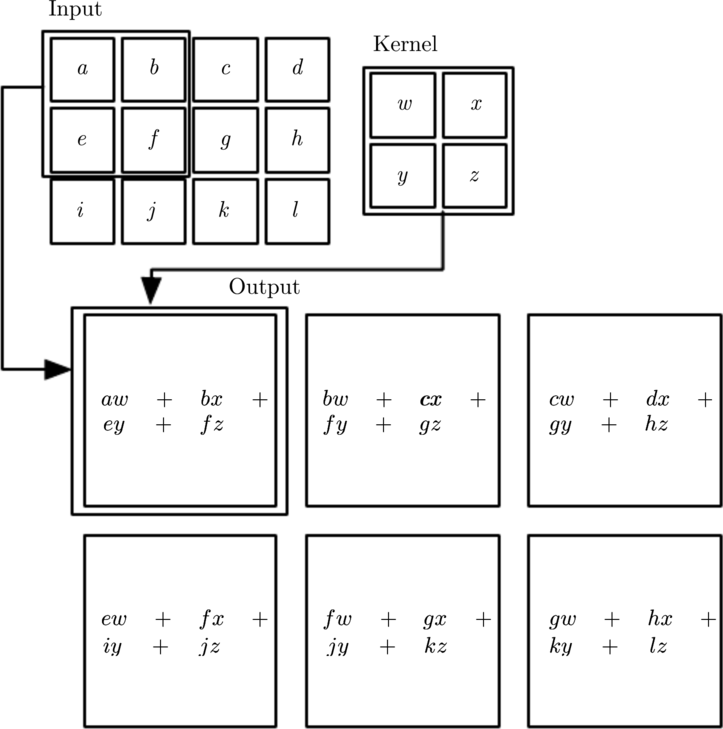
\includegraphics[scale=0.5]{images/70.png}}
\else
\centerline{\includegraphics{Chapter9/figures/conv_2d}}
\fi
\caption{一个2维卷积的例子(没有对核进行翻转)。
我们限制只对核完全处在图像中的位置进行输出,在一些上下文中称为``\gls{valid}''卷积。
我们用画有箭头的盒子来说明输出张量的左上角元素是如何通过对输入张量相应的左上角区域应用核进行卷积得到的。}
\label{fig:chap9_conv_2d}
\end{figure}

离散卷积可以看作矩阵的乘法,然而,这个矩阵的一些元素被限制为必须和另外一些元素相等。
例如对于单变量的离散卷积,矩阵每一行中的元素都与上一行对应位置平移一个单位的元素相同。
这种矩阵叫做\firstgls{Toeplitz_matrix}。
对于二维情况,卷积对应着一个\firstgls{doubly_block_circulant_matrix}。
%这里不是很理解双重分块循环矩阵
除了这些元素相等的限制以外,卷积通常对应着一个非常稀疏的矩阵(一个几乎所有元素都为零的矩阵)。
这是因为核的大小通常要远小于输入图像的大小。任何一个使用矩阵乘法但是并不依赖矩阵结构的特殊性质的神经网络算法,都适用于卷积运算,并且不需要对神经网络做出大的修改。
典型的\gls{CNN}为了更有效地处理大规模输入,确实使用了一些专门化的技巧,但这些在理论分析方面并不是严格必要的。

% -- 324 --
 
\section{动机}
\label{sec:motivation}

卷积运算通过三个重要的思想来帮助改进机器学习系统:\firstgls{sparse_interactions}、\firstgls{parameter_sharing}、\firstgls{equivariant_representations}。
另外,卷积提供了一种处理大小可变的输入的方法。
我们下面依次介绍这些思想。

传统的神经网络使用矩阵乘法来建立输入与输出的连接关系。%\footnote{译者注:这里可以粗略地理解为输入$\times$参数矩阵=输出。}
其中,参数矩阵中每一个单独的参数都描述了一个输入单元与一个输出单元间的交互。
这意味着每一个输出单元与每一个输入单元都产生交互。
然而,\gls{convolutional_network}具有\firstgls{sparse_interactions}(也叫做\firstgls{sparse_connectivity}或者\firstgls{sparse_weights})的特征。
这是使核的大小远小于输入的大小来达到的。
举个例子,当处理一张图像时,输入的图像可能包含成千上万个像素点,但是我们可以通过只占用几十到上百个像素点的核来检测一些小的有意义的特征,例如图像的边缘。
这意味着我们需要存储的参数更少,不仅减少了模型的存储需求,而且提高了它的统计效率。
这也意味着为了得到输出我们只需要更少的计算量。
这些效率上的提高往往是很显著的。
如果有$m$个输入和$n$个输出,那么矩阵乘法需要$m \times n$个参数并且相应算法的时间复杂度为$O(m\times n)$(对于每一个例子)。
如果我们限制每一个输出拥有的连接数为$k$,那么稀疏的连接方法只需要$k\times n$个参数以及$O(k\times n)$的运行时间。
在很多实际应用中,只需保持$k$比$m$小几个数量级,就能在机器学习的任务中取得好的表现。
\gls{sparse_connectivity}的图形化解释如\figref{fig:chap9_area_of_effect}和\figref{fig:chap9_receptive_field}所示。
在深度\gls{convolutional_network}中,处在网络深层的单元可能与绝大部分输入是\emph{间接}交互的,如\figref{fig:chap9_deep_receptive_field}所示。
这允许网络可以通过只描述\gls{sparse_interactions}的基石来高效地描述多个变量的复杂交互。
% fig 9.2
\begin{figure}[!htb]
\ifOpenSource
\centerline{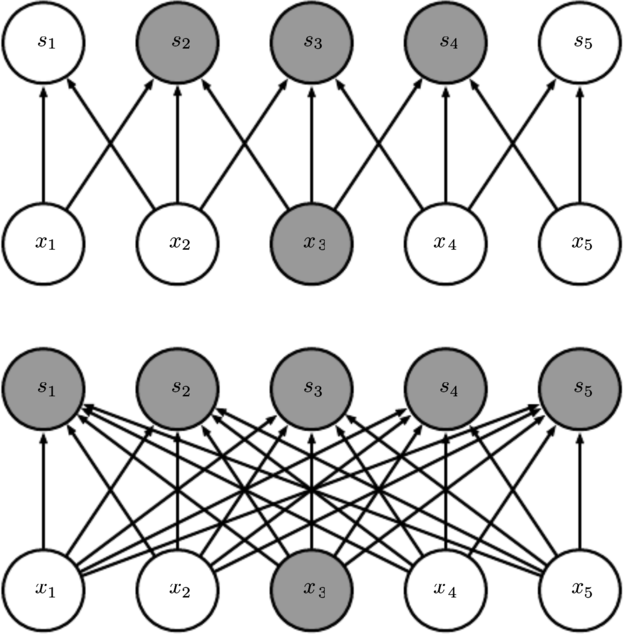
\includegraphics[scale=0.5]{images/71.png}}
\else
\centerline{\includegraphics{Chapter9/figures/area_of_effect}}
\fi
\captionsetup{singlelinecheck=off}
\caption[Caption for LOF]{\gls{sparse_connectivity},对每幅图从下往上看。
我们强调了一个输入单元$x_3$以及在$\Vs$中受该单元影响的输出单元。
\emph{(上)}当$\Vs$是由核宽度为3的卷积产生时,只有三个输出受到$\Vx$的影响\protect\footnotemark。
\emph{(下)}当$\Vs$是由矩阵乘法产生时,连接不再是稀疏的,所以所有的输出都会受到$x_3$的影响。}
\label{fig:chap9_area_of_effect}
\end{figure}
% \footnotetext{译者注:译者认为此处应当是$x_3$。}

% fig 9.3
\begin{figure}[!htb]
\ifOpenSource
\centerline{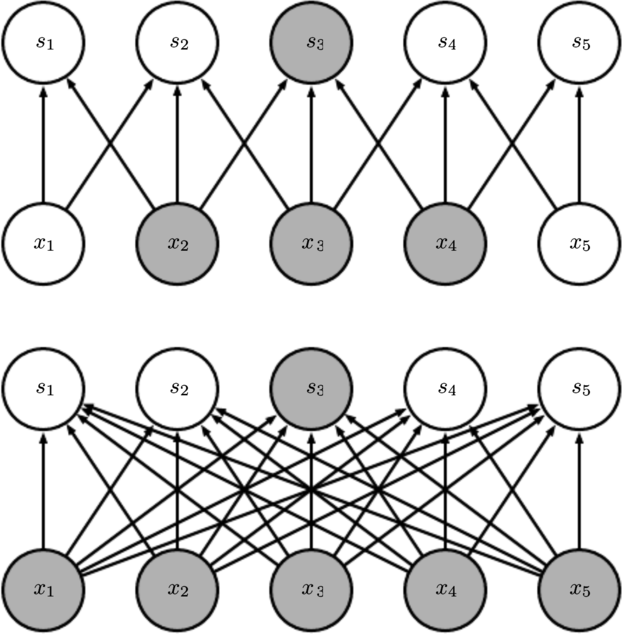
\includegraphics[scale=0.5]{images/72.png}}
\else
\centerline{\includegraphics{Chapter9/figures/receptive_field}}
\fi
\captionsetup{singlelinecheck=off}
\caption[Caption for LOF]{\gls{sparse_connectivity},对每幅图从上往下看。
我们强调了一个输出单元$s_3$以及$\Vx$中影响该单元的输入单元。
这些单元被称为$s_3$的\firstgls{receptive_field}\protect\footnotemark。
\emph{(上)}当$\Vs$是由核宽度为3的卷积产生时,只有三个输入影响$s_3$。
\emph{(下)}当$\Vs$是由矩阵乘法产生时,连接不再是稀疏的,所以所有的输入都会影响$s_3$。}
\label{fig:chap9_receptive_field}
\end{figure}
%\footnotetext{译者注:在生物中称之为``感受野''。}

% fig 9.4
\begin{figure}[!htb]
\ifOpenSource
\centerline{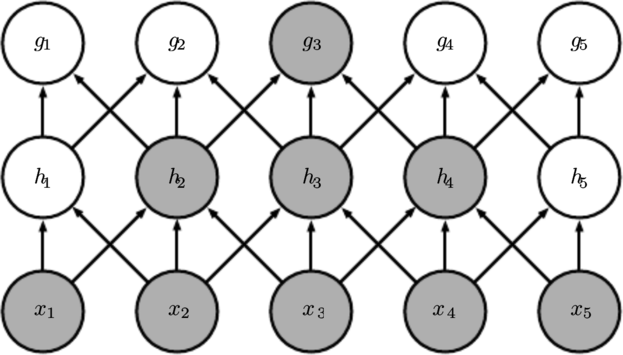
\includegraphics[scale=0.5]{images/73.png}}
\else
\centerline{\includegraphics{Chapter9/figures/deep_receptive_field}}
\fi
\caption{处于\gls{convolutional_network}更深的层中的单元,它们的\gls{receptive_field}要比处在浅层的单元的\gls{receptive_field}更大。
如果网络还包含类似\gls{stride}卷积(\figref{fig:chap9_stride_conv})或者\gls{pooling}(\secref{sec:pooling})之类的结构特征,这种效应会加强。
这意味着在\gls{convolutional_network}中尽管\emph{直接}连接都是很稀疏的,但处在更深的层中的单元可以\emph{间接地}连接到全部或者大部分输入图像。}
\label{fig:chap9_deep_receptive_field}
\end{figure}

% -- 325 --
 
\firstgls{parameter_sharing}是指在一个模型的多个函数中使用相同的参数。
在传统的神经网络中,当计算一层的输出时,权重矩阵的每一个元素只使用一次,当它乘以输入的一个元素后就再也不会用到了。
作为\gls{parameter_sharing}的同义词,我们可以说一个网络含有\firstgls{tied_weights},因为用于一个输入的权重也会被绑定在其他的权重上。
在\gls{CNN}中,核的每一个元素都作用在输入的每一位置上(是否考虑边界像素取决于对边界决策的设计)。
卷积运算中的\gls{parameter_sharing}保证了我们只需要学习一个参数集合,而不是对于每一位置都需要学习一个单独的参数集合。
这虽然没有改变\gls{forward_propagation}的运行时间(仍然是$O(k\times n)$),但它显著地把模型的存储需求降低至$k$个参数,并且$k$通常要比$m$小很多个数量级。
因为$m$ 和$n$通常有着大致相同的大小,$k$在实际中相对于$m\times n$是很小的。
因此,卷积在存储需求和统计效率方面极大地优于稠密矩阵的乘法运算。
\figref{fig:chap9_parameter_sharing}演示了\gls{parameter_sharing}是如何实现的。
% fig 9.5
\begin{figure}[!htb]
\ifOpenSource
\centerline{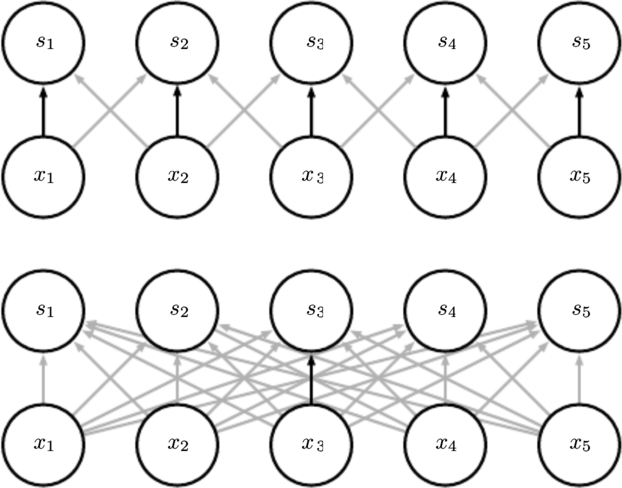
\includegraphics[scale=0.5]{images/74.png}}
\else
\centerline{\includegraphics{Chapter9/figures/parameter_sharing}}
\fi
\caption{\gls{parameter_sharing}。
黑色箭头表示在两个不同的模型中使用了特殊参数的连接。
\emph{(上)}黑色箭头表示在卷积模型中对3元素核的中间元素的使用。
因为\gls{parameter_sharing},这个单独的参数被用于所有的输入位置。
\emph{(下)}这个单独的黑色箭头表示在全连接模型中对权重矩阵的中间元素的使用。
这个模型没有使用\gls{parameter_sharing},所以参数只使用了一次。}
\label{fig:chap9_parameter_sharing}
\end{figure}
% -- 326 --
 
% -- 327 --
 
作为前两条原则的一个实际例子,\figref{fig:chap9_efficiency_of_edge_detection}说明了\gls{sparse_connectivity}和\gls{parameter_sharing}是如何显著提高线性函数在一张图像上进行边缘检测的效率的。
% fig 9.6
\begin{figure}
\ifOpenSource
\centerline{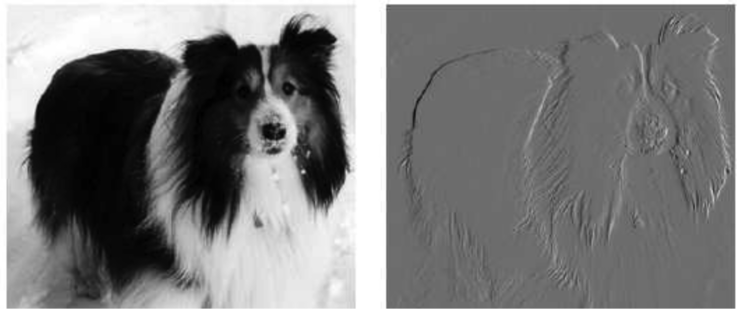
\includegraphics[scale=0.5]{images/75.png}}
\else
\centering    
\subfigure{ \label{fig:chap9_efficiency_of_edge_detection_a}     
\includegraphics[width=0.35\textwidth]{Chapter9/figures/sundance.png}}     
\subfigure{ \label{fig:chap9_efficiency_of_edge_detection_b}     
\includegraphics[width=0.35\textwidth]{Chapter9/figures/edges.png}}     
\fi
\captionsetup{singlelinecheck=off}
\caption{边缘检测的效率。
右边的图像是通过先获得原始图像中的每个像素,然后减去左边相邻像素的值而形成的。
这个操作给出了输入图像中所有垂直方向上的边缘的强度,对目标检测来说是有用的。
两个图像的高度均为280个像素。
输入图像的宽度为320个像素,而输出图像的宽度为319个像素。
这个变换可以通过包含两个元素的卷积核来描述,使用卷积需要$319\times 280\times 3 = 267,960$次浮点运算(每个输出像素需要两次乘法和一次加法)。
为了用矩阵乘法描述相同的变换,需要一个包含$320\times 280\times 319\times 280$个或者说超过80亿个元素的矩阵,这使得卷积对于表示这种变换更有效40亿倍。
直接运行矩阵乘法的算法将执行超过160亿次浮点运算,这使得卷积在计算上大约有60,000倍的效率。
当然,矩阵的大多数元素将为零。
如果我们只存储矩阵的非零元,则矩阵乘法和卷积都需要相同数量的浮点运算来计算。
矩阵仍然需要包含$2\times 319\times 280=178,640$个元素。
将小的局部区域上的相同线性变换应用到整个输入上,卷积是描述这种变换的极其有效的方法。
照片来源:Paula Goodfellow。}   
\label{fig:chap9_efficiency_of_edge_detection}     
\end{figure}
% -- 328 --
 
对于卷积,\gls{parameter_sharing}的特殊形式使得神经网络层具有对平移\firstgls{equivariance}的性质。
如果一个函数满足输入改变,输出也以同样的方式改变这一性质,我们就说它是等变(equivariant)的。
特别地,如果函数$f(x)$与$g(x)$满足$f(g(x))= g(f(x))$,我们就说$f(x)$对于变换$g$具有等变性。
对于卷积来说,如果令$g$是输入的任意平移函数,那么卷积函数对于$g$具有等变性。
举个例子,令$I$表示图像在整数坐标上的亮度函数,$g$表示图像函数的变换函数(把一个图像函数映射到另一个图像函数的函数)使得$I' = g(I)$,其中图像函数$I'$满足$I'(x,y) = I(x-1, y)$。
这个函数把$I$中的每个像素向右移动一个单位。
如果我们先对$I$进行这种变换然后进行卷积操作所得到的结果,与先对$I$进行卷积然后再对输出使用平移函数$g$得到的结果是一样的\footnote{译者注:原文将此处误写成了$I'$。} 。%译者注
当处理时间序列数据时,这意味着通过卷积可以得到一个由输入中出现不同特征的时刻所组成的时间轴。
如果我们把输入中的一个事件向后延时,在输出中仍然会有完全相同的表示,只是时间延后了。
图像与之类似,卷积产生了一个2维映射来表明某些特征在输入中出现的位置。
如果我们移动输入中的对象,它的表示也会在输出中移动同样的量。
当处理多个输入位置时,一些作用在邻居像素的函数是很有用的。
例如在处理图像时,在\gls{convolutional_network}的第一层进行图像的边缘检测是很有用的。
相同的边缘或多或少地散落在图像的各处,所以应当对整个图像进行\gls{parameter_sharing}。
但在某些情况下,我们并不希望对整幅图进行\gls{parameter_sharing}。
例如,在处理已经通过剪裁而使其居中的人脸图像时,我们可能想要提取不同位置上的不同特征(处理人脸上部的部分网络需要去搜寻眉毛,处理人脸下部的部分网络就需要去搜寻下巴了)。

% -- 329 --
 
卷积对其他的一些变换并不是天然等变的,例如对于图像的放缩或者旋转变换,需要其他的一些机制来处理这些变换。

最后,一些不能被传统的由(固定大小的)矩阵乘法定义的神经网络处理的特殊数据,可能通过卷积神经网络来处理,我们将在\secref{sec:data_types}中进行讨论。

\section{\glsentrytext{pooling}}
\label{sec:pooling}

\gls{convolutional_network}中一个典型层包含三级(如\figref{fig:chap9_conv_layer}所示)。
在第一级中,这一层并行地计算多个卷积产生一组线性激活响应。
在第二级中,每一个线性激活响应将会通过一个非线性的激活函数,例如\gls{rectified_linear}激活函数。
这一级有时也被称为\firstgls{detector_stage}。
在第三级中,我们使用\firstgls{pooling_funciton}来进一步调整这一层的输出。
% fig 9.7
\begin{figure}[!htb]
\ifOpenSource
\centerline{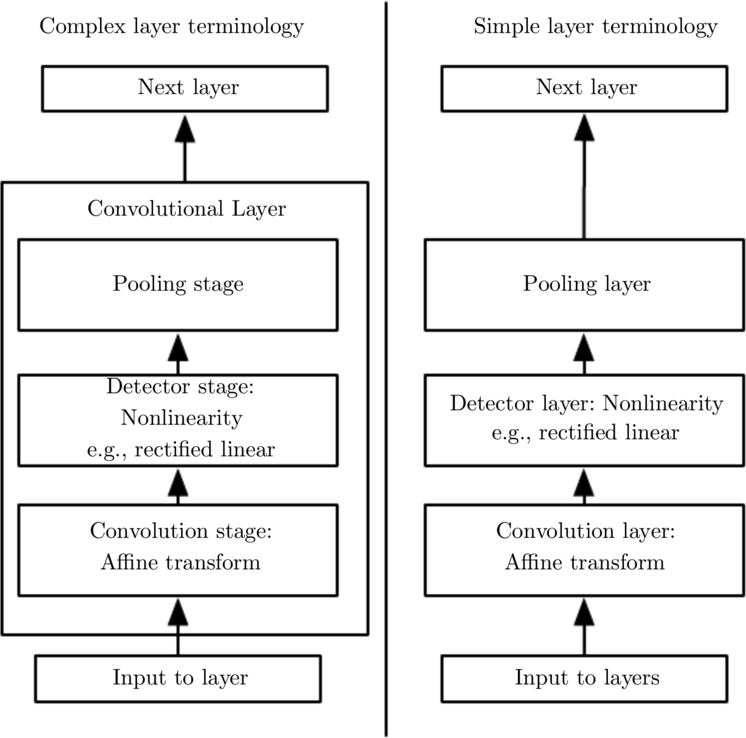
\includegraphics[scale=0.5]{images/76.png}}
\else
\centerline{\includegraphics{Chapter9/figures/conv_layer}}
\fi
\caption{一个典型\gls{CNN}层的组件。
有两组常用的术语用于描述这些层。
\emph{(左)}在这组术语中,\gls{convolutional_network}被视为少量相对复杂的层,每层具有许多``级''。
在这组术语中,核张量与网络层之间存在一一对应关系。
在本书中,我们通常使用这组术语。
\emph{(右)}在这组术语中,\gls{convolutional_network}被视为更多数量的简单层;每一个处理步骤都被认为是一个独立的层。
这意味着不是每一``层''都有参数。}
\label{fig:chap9_conv_layer}
\end{figure}

\gls{pooling}函数使用某一位置的相邻输出的总体统计特征来代替网络在该位置的输出。
例如,\firstgls{max_pooling}函数\citep{zhou1988computation}给出相邻矩形区域内的最大值。
其他常用的\gls{pooling}函数包括相邻矩形区域内的平均值、$L^2$范数以及基于据中心像素距离的加权平均函数。

% -- 330 --
 
不管采用什么样的\gls{pooling}函数,当输入作出少量平移时,\gls{pooling}能够帮助输入的表示近似\firstgls{invariant}。
对于平移的不变性是指当我们对输入进行少量平移时,经过\gls{pooling}函数后的大多数输出并不会发生改变。
\figref{fig:chap9_max_pool_invariance}用了一个例子来说明这是如何实现的。
\emph{局部平移不变性是一个很有用的性质,尤其是当我们关心某个特征是否出现而不关心它出现的具体位置时}。
例如,当判定一张图像中是否包含人脸时,我们并不需要知道眼睛的精确像素位置,我们只需要知道有一只眼睛在脸的左边,有一只在右边就行了。
但在一些其他领域,保存特征的具体位置却很重要。
例如当我们想要寻找一个由两条边相交而成的拐角时,我们就需要很好地保存边的位置来判定它们是否相交。
% fig 9.8
\begin{figure}[!htb]
\ifOpenSource
\centerline{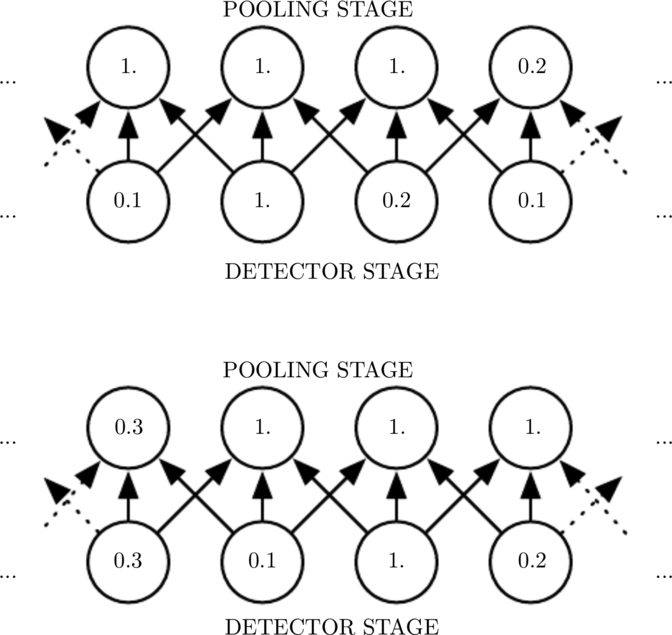
\includegraphics[scale=0.5]{images/77.png}}
\else
\centerline{\includegraphics{Chapter9/figures/max_pool_invariance}}
\fi
\caption{\gls{max_pooling}引入了不变性。
\emph{(上)}卷积层中间输出的视图。
下面一行显示非线性的输出。
上面一行显示\gls{max_pooling}的输出,每个\gls{pool}的宽度为三个像素并且\gls{pooling}区域的\gls{stride}为一个像素。
\emph{(下)}相同网络的视图,不过对输入右移了一个像素。
下面一行的所有值都发生了改变,但上面一行只有一半的值发生了改变,这是因为\gls{max_pooling}单元只对周围的最大值比较敏感,而不是对精确的位置。}
\label{fig:chap9_max_pool_invariance}
\end{figure}

% -- 331 --
 
使用\gls{pooling}可以看作是增加了一个无限强的先验:这一层学得的函数必须具有对少量平移的不变性。
当这个假设成立时,\gls{pooling}可以极大地提高网络的统计效率。

对空间区域进行\gls{pooling}产生了平移不变性,但当我们对分离参数的卷积的输出进行\gls{pooling}时,特征能够学得应该对于哪种变换具有不变性(如\figref{fig:chap9_learned_rotation}所示)。
% fig 9.9
\begin{figure}[!htb]
\ifOpenSource
\centerline{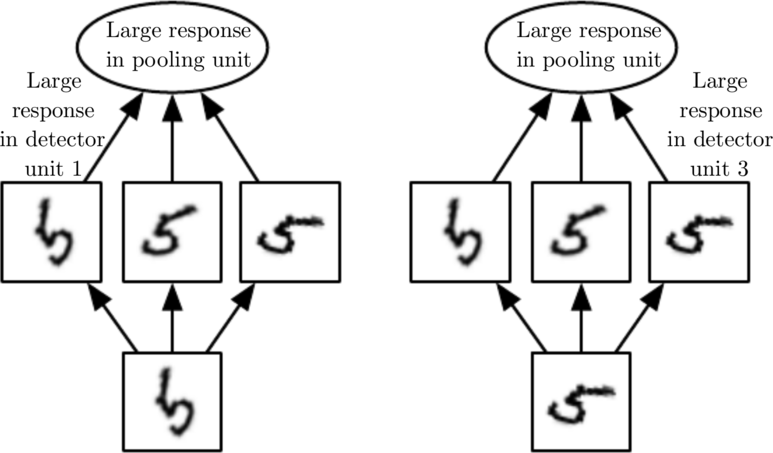
\includegraphics[scale=0.5]{images/78.png}}
\else
\centerline{\includegraphics{Chapter9/figures/learned_rotation}}
\fi
\caption{学习不变性的示例。
使用分离的参数学得多个特征,再使用\gls{pooling}单元进行\gls{pooling},可以学得对输入的某些变换的不变性。
这里我们展示了用三个学得的过滤器和一个\gls{max_pooling}单元可以学得对旋转变换的不变性。
这三个过滤器都旨在检测手写的数字5。
每个过滤器尝试匹配稍微不同方向的5。
当输入中出现5时,相应的过滤器会匹配它并且在探测单元中引起大的激活。
然后,无论哪个探测单元被激活,\gls{max_pooling}单元都具有大的激活。
我们在这里演示了网络如何处理两个不同的输入,这导致两个不同的探测单元被激活,然而对\gls{pooling}单元的影响大致相同。
这个原则在\,\gls{maxout}\,网络\citep{Goodfellow-et-al-ICML2013}和其他卷积网络中更有影响。
空间位置上的\gls{max_pooling}对于平移是天然不变的;这种多通道方法只在学习其他变换时是必要的。}
\label{fig:chap9_learned_rotation}
\end{figure}

% -- 332 --
 
因为\gls{pooling}综合了全部邻居的反馈,这使得\gls{pooling}单元少于探测单元成为可能,我们可以通过综合\gls{pooling}区域的$k$个像素的统计特征而不是单个像素来实现。
\figref{fig:chap9_pool_downsample}给出了一个例子。
这种方法提高了网络的计算效率,因为下一层少了约$k$ 倍的输入。
当下一层的参数数目是关于那一层输入大小的函数时(例如当下一层是全连接的基于矩阵乘法的网络层时),这种对于输入规模的减小也可以提高统计效率并且减少对于参数的存储需求。
% fig 9.10
\begin{figure}[!htb]
\ifOpenSource
\centerline{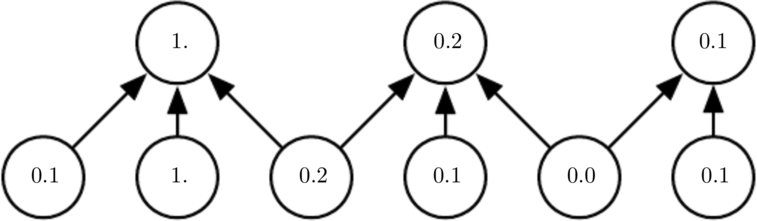
\includegraphics[scale=0.5]{images/79.png}}
\else
\centerline{\includegraphics{Chapter9/figures/pool_downsample}}
\fi
\caption{带有\gls{downsampling}的\gls{pooling}。
这里我们使用\gls{max_pooling},\gls{pool}的宽度为三并且\gls{pool}之间的\gls{stride}为二。
这使得表示的大小减少了一半,减轻了下一层的计算和统计负担。
注意到最右边的\gls{pooling}区域尺寸较小,但如果我们不想忽略一些探测单元的话就必须包含这个区域。}
\label{fig:chap9_pool_downsample}
\end{figure}

% -- 333 --
 
在很多任务中,\gls{pooling}对于处理不同大小的输入具有重要作用。
例如我们想对不同大小的图像进行分类时,分类层的输入必须是固定的大小,而这通常通过调整\gls{pooling}区域的偏置大小来实现,这样分类层总是能接收到相同数量的统计特征而不管最初的输入大小了。
例如,最终的\gls{pooling}层可能会输出四组综合统计特征,每组对应着图像的一个象限,而与图像的大小无关。

一些理论工作对于在不同情况下应当使用哪种\gls{pooling}函数给出了一些指导\citep{boureau-icml-10}。
将特征一起动态地\gls{pooling}也是可行的,例如,对于感兴趣特征的位置运行聚类算法\citep{boureau-iccv-11}。
这种方法对于每幅图像产生一个不同的\gls{pooling}区域集合。
另一种方法是先\emph{学习}一个单独的\gls{pooling}结构,再应用到全部的图像中\citep{jia2012beyond}。

\gls{pooling}可能会使得一些利用自顶向下信息的神经网络结构变得复杂,例如\gls{BM}和\gls{AE}。
这些问题将在\chapref{part:deep_learning_research}中当我们遇到这些类型的网络时进一步讨论。
\gls{CBM}中的\gls{pooling}出现在\secref{sec:convolutional_boltzmann_machines}。
一些可微网络中需要的在\gls{pooling}单元上进行的类逆运算将在\secref{sec:convolutional_generative_networks}中讨论。

\figref{fig:chap9_cnn_classifier}给出了一些使用卷积和\gls{pooling}操作的用于分类的完整\gls{convolutional_network}结构的例子。
% fig 9.11
\begin{figure}[!htb]
\ifOpenSource
\centerline{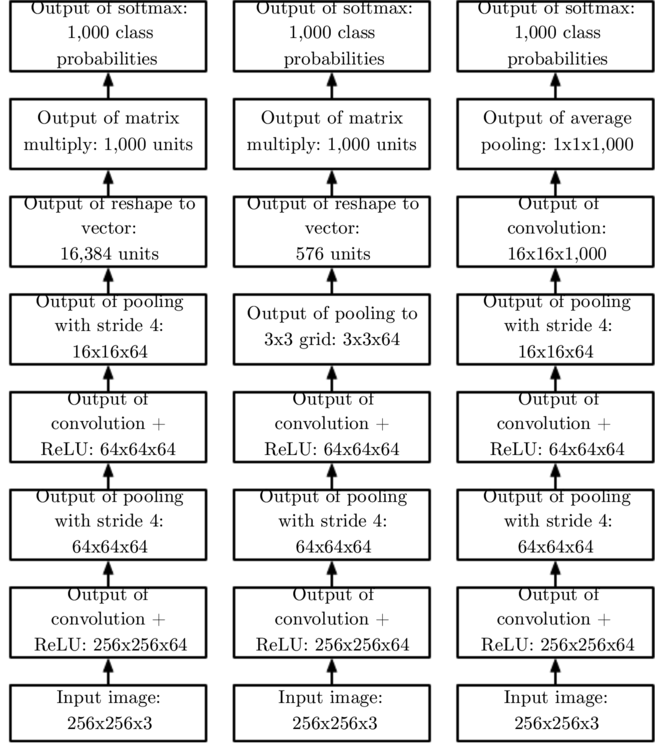
\includegraphics[scale=0.5]{images/80.png}}
\else
\centerline{\includegraphics{Chapter9/figures/cnn_classifier}}
\fi
\caption{\gls{convolutional_network}用于分类的结构示例。
本图中使用的具体\gls{stride}和深度并不建议实际使用;它们被设计得非常浅以适合页面。
实际的\gls{convolutional_network}还常常涉及大量的分支,不同于这里为简单起见所使用的链式结构。
\emph{(左)}处理固定大小的图像的\gls{convolutional_network}。
在卷积层和\gls{pooling}层几层交替之后,卷积特征映射的张量被重新变形以展平空间维度。
网络的其余部分是一个普通的前馈网络分类器,如\chapref{chap:deep_feedforward_networks}所述。
\emph{(中)}处理大小可变的图像的\gls{convolutional_network},但仍保持全连接的部分。
该网络使用具有可变大小但是数量固定的\gls{pool}的\gls{pooling}操作,以便向网络的全连接部分提供固定576个单位大小的向量。 
\emph{(右)}没有任何全连接权重层的\gls{convolutional_network}。
相对的,最后的卷积层为每个类输出一个特征映射。
该模型可能会用来学习每个类出现在每个空间位置的可能性的映射。
将特征映射进行平均得到的单个值,提供了顶部softmax分类器的变量。}
\label{fig:chap9_cnn_classifier}
\end{figure}

\section{卷积与\glsentrytext{pooling}作为一种无限强的先验}
\label{sec:convolution_and_pooling_as_an_infinitely_strong_prior}

回忆一下\secref{sec:capacity_overfitting_and_underfitting}中\firstgls{prior_probability_distribution}的概念。
这是一个模型参数的概率分布,它刻画了在我们看到数据之前我们认为什么样的模型是合理的信念。

% -- 334 --
 
先验被认为是强或者弱取决于先验中概率密度的集中程度。
弱先验具有较高的熵值,例如方差很大的\gls{gaussian_distribution}。这样的先验允许数据对于参数的改变具有或多或少的自由性。
强先验具有较低的熵值,例如方差很小的\gls{gaussian_distribution}。这样的先验在决定参数最终取值时起着更加积极的作用。

一个无限强的先验需要对一些参数的概率置零并且完全禁止对这些参数赋值,无论数据对于这些参数的值给出了多大的支持。

我们可以把\gls{convolutional_network}类比成全连接网络,但对于这个全连接网络的权重有一个无限强的先验。
这个无限强的先验是说一个\gls{hidden_unit}的权重必须和它邻居的权重相同,但可以在空间上移动。
这个先验也要求除了那些处在\gls{hidden_unit}的小的空间连续的\gls{receptive_field}内的权重以外,其余的权重都为零。
%这样翻译对吗?其实这里加个图更好
总之,我们可以把卷积的使用当作是对网络中一层的参数引入了一个无限强的\gls{prior_probability_distribution}。
这个先验说明了该层应该学得的函数只包含局部连接关系并且对平移具有等变性。
类似的,使用\gls{pooling}也是一个无限强的先验:每一个单元都具有对少量平移的不变性。

当然,把\gls{CNN}当作一个具有无限强先验的全连接网络来实现会导致极大的计算浪费。
但把\gls{CNN}想成具有无限强先验的全连接网络可以帮助我们更好地洞察\gls{CNN}是如何工作的。

其中一个关键的洞察是卷积和\gls{pooling}可能导致\gls{underfitting}。
与任何其他先验类似,卷积和\gls{pooling}只有当先验的假设合理且正确时才有用。
如果一项任务依赖于保存精确的空间信息,那么在所有的特征上使用\gls{pooling}将会增大训练误差。
一些\gls{convolutional_network}结构~\citep{Szegedy-et-al-arxiv2014}为了既获得具有较高不变性的特征又获得当平移不变性不合理时不会导致\gls{underfitting}的特征,被设计成在一些通道上使用\gls{pooling}而在另一些通道上不使用。
当一项任务涉及到要对输入中相隔较远的信息进行合并时,那么卷积所利用的先验可能就不正确了。

另一个关键洞察是当我们比较卷积模型的统计学习表现时,只能以基准中的其他卷积模型作为比较的对象。
其他不使用卷积的模型即使我们把图像中的所有像素点都置换后依然有可能进行学习。
对于许多图像数据集,还有一些分别的基准,有些是针对那些具有\firstgls{permutation_invariant}并且必须通过学习发现拓扑结构的模型,还有一些是针对模型设计者将空间关系的知识植入了它们的模型。

% -- 336 --

\section{基本卷积函数的变体}
\label{sec:variants_of_the_basic_convolution_function}

当在神经网络的上下文中讨论卷积时,我们通常不是特指数学文献中使用的那种标准的离散卷积运算。
实际应用中的函数略有不同。
这里我们详细讨论一下这些差异,并且对神经网络中用到的函数的一些重要性质进行重点说明。

首先,当我们提到神经网络中的卷积时,我们通常是指由多个并行卷积组成的运算。
这是因为具有单个核的卷积只能提取一种类型的特征,尽管它作用在多个空间位置上。
我们通常希望网络的每一层能够在多个位置提取多种类型的特征。

另外,输入通常也不仅仅是实值的网格,而是由一系列观测数据的向量构成的网格。
例如,一幅彩色图像在每一个像素点都会有红绿蓝三种颜色的亮度。
在多层的\gls{convolutional_network}中,第二层的输入是第一层的输出,通常在每个位置包含多个不同卷积的输出。
当处理图像时,我们通常把卷积的输入输出都看作是3维的张量,其中一个索引用于标明不同的通道(例如红绿蓝),另外两个索引标明在每个通道上的空间坐标。
软件实现通常使用批处理模式,所以实际上会使用4维的张量,第四维索引用于标明批处理中不同的实例,但我们为简明起见这里忽略批处理索引。

因为\gls{convolutional_network}通常使用多通道的卷积,所以即使使用了核翻转, 也不一定保证网络的线性运算是可交换的。
只有当其中的每个运算的输出和输入具有相同的通道数时,这些多通道的运算才是可交换的。。

假定我们有一个4维的核张量$\TSK$,它的每一个元素是$\TEK_{i,j,k,l}$,表示输出中处于通道$i$的一个单元和输入中处于通道$j$中的一个单元的连接强度,并且在输出单元和输入单元之间有$k$行$l$列的偏置。
假定我们的输入由观测数据$\TSV$组成,它的每一个元素是$\TEV_{i,j,k}$,表示处在通道$i$中第$j$行第$k$列的值。
假定我们的输出$\TSZ$和输入$\TSV$具有相同的形式。
如果输出$\TSZ$是通过对$\TSK$和$\TSV$进行卷积而不涉及翻转$\TSK$得到的,那么
\begin{equation}
\TEZ_{i,j,k} = \sum_{l,m,n} \TEV_{l, j+m-1, k+n-1} \TEK_{i,l,m,n},
\end{equation}
这里对所有的$l$,$m$和$n$进行求和是对所有(在求和式中)有效的张量索引的值进行求和。
在线性代数中,向量的索引通常从1开始,这就是上述公式中$-1$的由来。
但是像C或Python这类编程语言索引通常从0开始,这使得上述公式可以更加简洁。

% -- 337 --
 
我们有时会希望跳过核中的一些位置来降低计算的开销(相应的代价是提取特征没有先前那么好了)。
我们可以把这一过程看作是对全卷积函数输出的下采样(downsampling)。
如果我们只想在输出的每个方向上每间隔$s$个像素进行采样,那么我们可以定义一个下采样卷积函数$c$使得
\begin{equation}
\TEZ_{i,j,k} = c(\TSK, \TSV, s)_{i,j,k} = \sum_{l,m,n} [\TEV_{l,(j-1)\times s+m, (k-1)\times s +n,}
 \TEK_{i,l,m,n}].
 \label{eq:9.8}
\end{equation}
我们把$s$称为下采样卷积的\firstgls{stride}。
当然也可以对每个移动方向定义不同的步幅。
\figref{fig:chap9_stride_conv}演示了一个实例。
% fig 9.12
\begin{figure}[!htb]
\ifOpenSource
\centerline{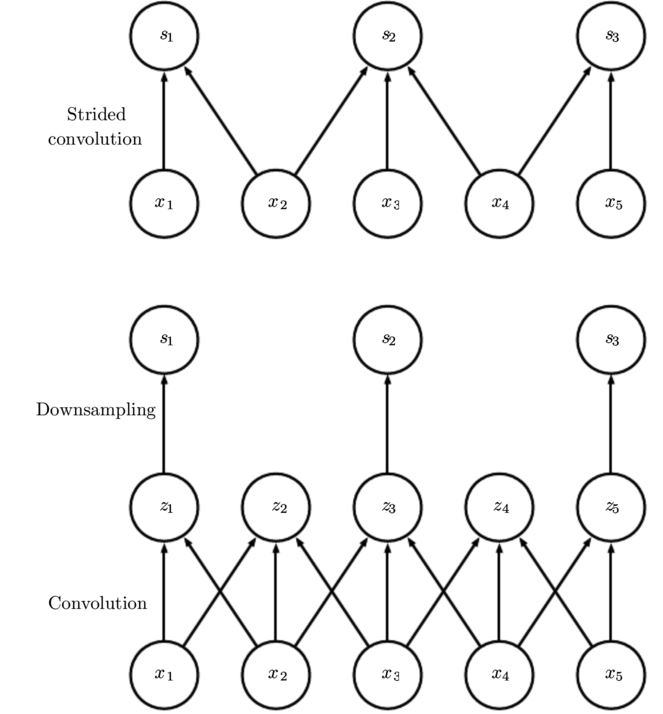
\includegraphics[scale=0.5]{images/81.png}}
\else
\centerline{\includegraphics{Chapter9/figures/stride_conv}}
\fi
\caption{带有\gls{stride}的卷积。
在这个例子中,我们的\gls{stride}为二。
\emph{(上)}\,在单个操作中实现的\gls{stride}为二的卷积。
\emph{(下)}\,\gls{stride}大于一个像素的卷积在数学上等价于单位\gls{stride}的卷积随后\gls{downsampling}。
显然,涉及\gls{downsampling}的两步法在计算上是浪费的,因为它计算了许多将被丢弃的值。}
\label{fig:chap9_stride_conv}
\end{figure}

在任何\gls{convolutional_network}的实现中都有一个重要性质,那就是能够隐含地对输入$\TSV$用零进行填充(pad)使得它加宽。
如果没有这个性质,\gls{representation}的宽度在每一层就会缩减,缩减的幅度是比核少一个像素这么多。
对输入进行零填充允许我们对核的宽度和输出的大小进行独立的控制。
如果没有零填充,我们就被迫面临二选一的局面,要么选择网络空间宽度的快速缩减,要么选择一个小型的核——这两种情境都会极大得限制网络的表示能力。
\figref{fig:chap9_zero_pad_shrink}给出了一个例子。
% fig 9.13
\begin{figure}[!htb]
\ifOpenSource
\centerline{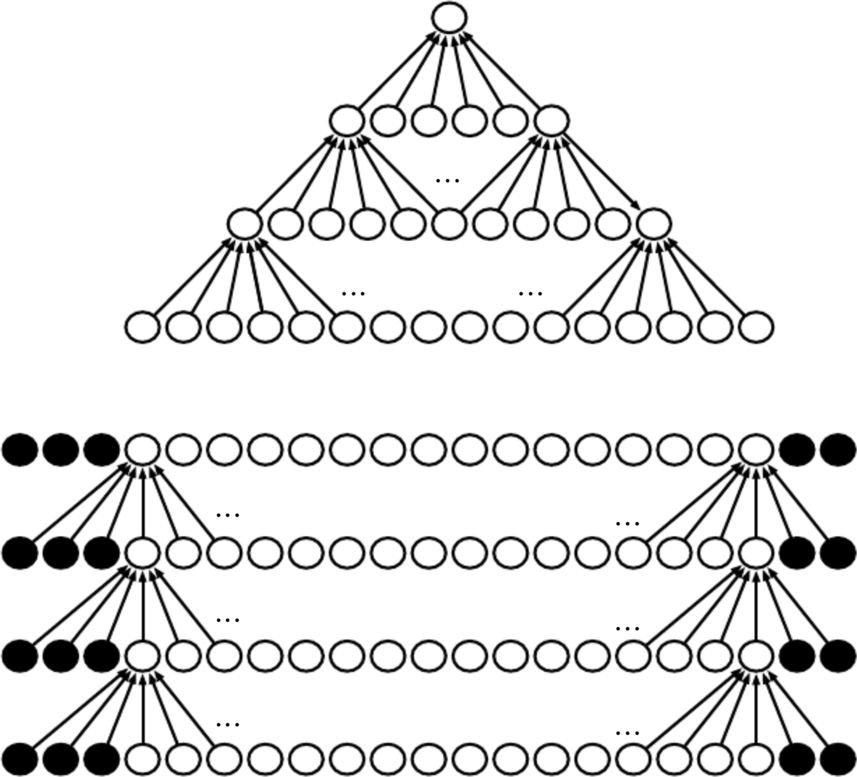
\includegraphics[scale=0.5]{images/82.png}}
\else
\centerline{\includegraphics{Chapter9/figures/zero_pad_shrink}}
\fi
\caption{零填充对网络大小的影响。
考虑一个\gls{convolutional_network},每层有一个宽度为六的核。 
在这个例子中,我们不使用任何\gls{pooling},所以只有卷积操作本身缩小网络的大小。
\emph{(上)}在这个卷积网络中,我们不使用任何隐含的零填充。
这使得表示在每层缩小五个像素。
从十六个像素的输入开始,我们只能有三个卷积层,并且最后一层不能移动核,所以可以说只有两层是真正的卷积层。
可以通过使用较小的核来减缓收缩速率,但是较小的核表示能力不足,并且在这种结构中一些收缩是不可避免的。
\emph{(下)}通过向每层添加五个隐含的零,我们防止了表示随深度收缩。
这允许我们设计一个任意深的卷积网络。}
\label{fig:chap9_zero_pad_shrink}
\end{figure}

有三种零填充设定的情况值得注意。
第一种是无论怎样都不使用零填充的极端情况,并且卷积核只允许访问那些图像中能够完全包含整个核的位置。
在MATLAB的术语中,这称为\firstgls{valid}卷积。
在这种情况下,输出的所有像素都是输入中相同数量像素的函数,这使得输出像素的表示更加规范。
然而,输出的大小在每一层都会缩减。
如果输入的图像宽度是$m$,核的宽度是$k$,那么输出的宽度就会变成$m-k+1$。
如果卷积核非常大的话缩减率会非常显著。
因为缩减数大于0,这限制了网络中能够包含的卷积层的层数。
当层数增加时,网络的空间维度最终会缩减到$1\times 1$,这种情况下增加的层就不可能进行有意义的卷积了。
第二种特殊的情况是只进行足够的零填充来保持输出和输入具有相同的大小。
在MATLAB的术语中,这称为\firstgls{same}卷积。
在这种情况下,只要硬件支持,网络就能包含任意多的卷积层,这是因为卷积运算不改变下一层的结构。。
然而,输入像素中靠近边界的部分相比于中间部分对于输出像素的影响更小。
这可能会导致边界像素存在一定程度的欠表示。
这使得第三种极端情况产生了,在MATLAB中称为\firstgls{full}卷积。
它进行了足够多的零填充使得每个像素在每个方向上恰好被访问了$k$次,最终输出图像的宽度为$m+k-1$。%\footnote{译者注:图\ref{fig:chap9_zero_pad_shrink}给出了\gls{valid}卷积和\gls{same}卷积的例子,这里对\gls{full}卷积略作说明:我们可以认为\gls{full}卷积是在输入的两端各填充$k-1$个零,使得输入的每个像素都恰好被核访问$k$次,最终得到的输出的宽度为$[m+2(k-1)]-k+1=m+k-1$}
在这种情况下,输出像素中靠近边界的部分相比于中间部分是更少像素的函数。
这将导致学得一个在卷积特征映射的所有位置都表现不错的单核更为困难。
通常零填充的最优数量(对于测试集的分类正确率)处于``\gls{valid}卷积''和``\gls{same}卷积''之间的某个位置。

% -- 338 --
 
% -- 339 --

在一些情况下,我们并不是真的想使用卷积,而是想用一些局部连接的网络层\citep{LeCun86,LeCun89a}。
在这种情况下,我们的\gls{MLP}对应的邻接矩阵是相同的,但每一个连接都有它自己的权重,用一个6维的张量$\TSW$来表示。
$\TSW$的索引分别是:输出的通道$i$,输出的行$j$和列$k$,输入的通道$l$,输入的行偏置$m$和列偏置$n$。
局部连接层的线性部分可以表示为
\begin{equation}
\TEZ_{i,j,k} = \sum_{l,m,n} [\TEV_{l, j+m-1, k+n-1} w_{i, j, k, l, m, n}]. %这里应该是$\TEW$?
\end{equation}
这有时也被称为\firstgls{unshared_convolution},因为它和具有一个小核的离散卷积运算很像,但并不横跨位置来共享参数。
图\ref{fig:chap9_local}比较了局部连接、卷积和全连接的区别。
% fig 9.14
\begin{figure}[!htb]
\ifOpenSource
\centerline{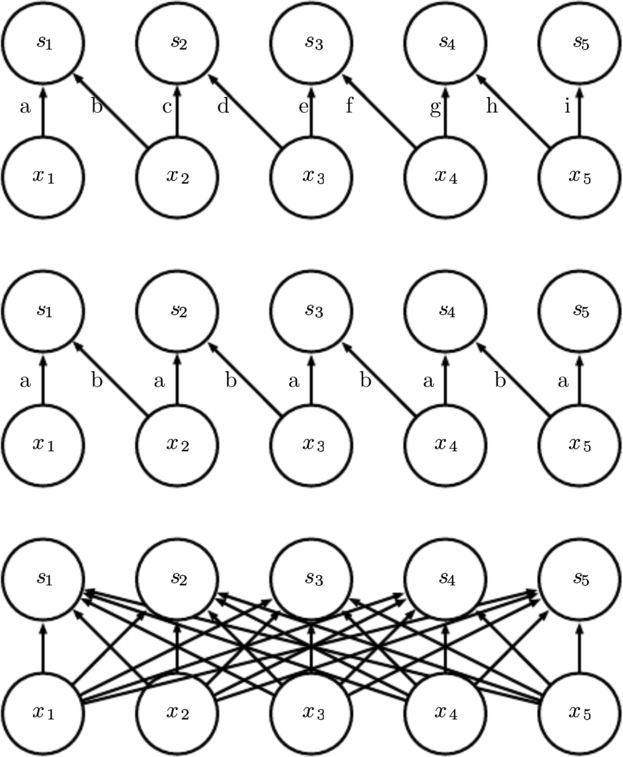
\includegraphics[scale=0.5]{images/83.png}}
\else
\centerline{\includegraphics{Chapter9/figures/local}}
\fi
\caption{局部连接,卷积和全连接的比较。
\emph{(上)}每一小片(接受域)有两个像素的局部连接层。
每条边用唯一的字母标记,来显示每条边都有自身的权重参数。
\emph{(中)}核宽度为两个像素的卷积层。
该模型与局部连接层具有完全相同的连接。
区别不在于哪些单元相互交互,而在于如何共享参数。
局部连接层没有\gls{parameter_sharing}。
正如用于标记每条边的字母重复出现所指示的,卷积层在整个输入上重复使用相同的两个权重。
\emph{(下)}全连接层类似于局部连接层,它的每条边都有其自身的参数(在该图中用字母明确标记的话就太多了)。 然而,它不具有局部连接层的连接受限的特征。}
\label{fig:chap9_local}
\end{figure}
 
% -- 340 --
 
当我们知道每一个特征都是一小块空间的函数并且相同的特征不会出现在所有的空间上时,局部连接层是很有用的。
例如,如果我们想要辨别一张图片是否是人脸图像时,我们只需要去寻找嘴是否在图像下半部分即可。

使用那些连接被更进一步限制的卷积或者局部连接层也是有用的,例如,限制每一个输出的通道$i$仅仅是输入通道$l$的一部分的函数时。
实现这种情况的一种通用方法是使输出的前$m$个通道仅仅连接到输入的前$n$个通道,输出的接下来的$m$个通道仅仅连接到输入的接下来的$n$个通道,以此类推。
\figref{fig:chap9_conv_groups}给出了一个例子。
对少量通道间的连接进行建模允许网络使用更少的参数,这降低了存储的消耗以及提高了统计效率,并且减少了前向和反向传播所需要的计算量。
这些目标的实现并没有减少\gls{hidden_unit}的数目。
% fig 9.15
\begin{figure}[!htb]
\ifOpenSource
\centerline{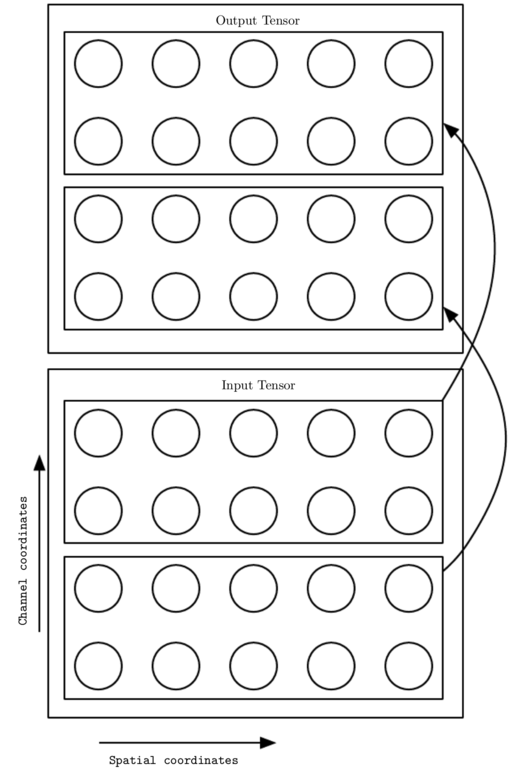
\includegraphics[scale=0.5]{images/84.png}}
\else
\centerline{\includegraphics{Chapter9/figures/conv_groups}}
\fi
\caption{\gls{convolutional_network}的前两个输出通道只和前两个输入通道相连,随后的两个输出通道只和随后的两个输入通道相连。}
\label{fig:chap9_conv_groups}
\end{figure}

\firstgls{tiled_convolution}\citep{Gregor+LeCun-2010,Le2010}对卷积层和局部连接层进行了折衷。
这里并不是对\emph{每一个}空间位置的权重集合进行学习,我们学习一组核使得当我们在空间移动时它们可以循环利用。
这意味着在近邻的位置上拥有不同的过滤器,就像局部连接层一样,但是对于这些参数的存储需求仅仅会增长常数倍,这个常数就是核的集合的大小,而不是整个输出的特征映射的大小。
\figref{fig:chap9_tiled}对局部连接层、\gls{tiled_convolution}和标准卷积进行了比较。
% fig 9.16
\begin{figure}[!htb]
\ifOpenSource
\centerline{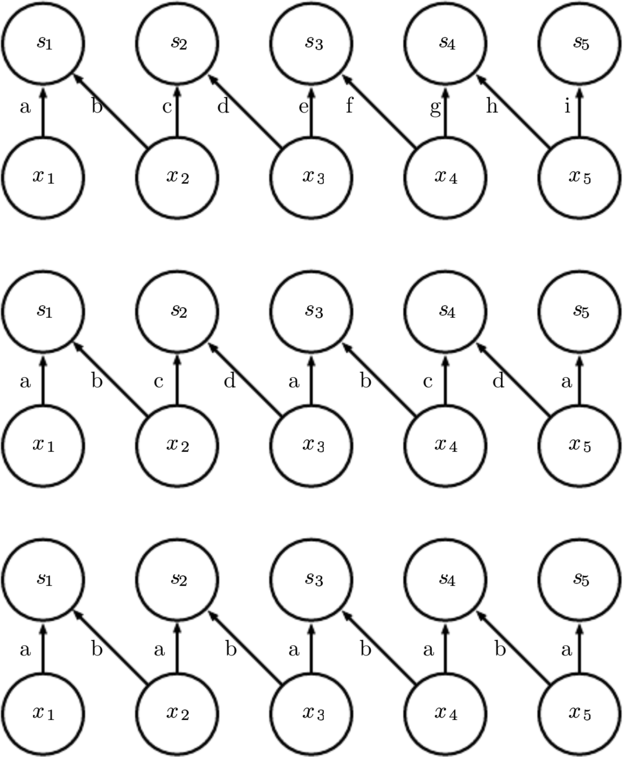
\includegraphics[scale=0.5]{images/85.png}}
\else
\centerline{\includegraphics{Chapter9/figures/tiled}}
\fi
\captionsetup{singlelinecheck=off}
\caption[.]{局部连接层、\gls{tiled_convolution}和标准卷积的比较。
当使用相同大小的核时,这三种方法在单元之间具有相同的连接。
此图是对使用两个像素宽的核的说明。
这三种方法之间的区别在于它们如何共享参数。
\emph{(上)}局部连接层根本没有共享参数。
我们对每个连接使用唯一的字母标记,来表明每个连接都有它自身的权重。
\emph{(中)}\gls{tiled_convolution}有$t$个不同的核。
这里我们说明$t=2$的情况。
其中一个核具有标记为``a''和``b''的边,而另一个具有标记为``c''和``d''的边。
每当我们在输出中右移一个像素后,我们使用一个不同的核。
这意味着,与局部连接层类似,输出中的相邻单元具有不同的参数。
与局部连接层不同的是,在我们遍历所有可用的$t$个核之后,我们循环回到了第一个核。
如果两个输出单元间隔$t$个步长的倍数,则它们共享参数。
\emph{(下)}传统卷积等效于$t=1$的\gls{tiled_convolution}。
它只有一个核,并且被应用到各个地方,我们在图中表示为在各处使用具有标记为``a''和``b''的边的核。}
\label{fig:chap9_tiled}
\end{figure}
 
% -- 341 --
 
为了用代数的方法定义\gls{tiled_convolution},令$\TSK$是一个6维的张量\footnote{译者注:原文将$\TSK$误写成了$k$。},其中的两维对应着输出映射中的不同位置。
$\TSK$在这里并没有对输出映射中的每一个位置使用单独的索引,输出的位置在每个方向上在$t$个不同的核组成的集合中进行循环。
如果$t$等于输出的宽度,这就是局部连接层了。
\begin{equation}
\TEZ_{i, j, k} = \sum_{l, m, n} \TEV_{l, j+m-1, k+n-1} \TEK_{i, l, m, n, j\% t +1, k\% t+1},
\end{equation}
这里百分号是取模运算,它的性质包括$t\% t =0, (t+1)\% t = 1$等等。
在每一维上使用不同的$t$可以很容易对这个方程进行扩展。
 
% -- 342 --
  
% -- 343 --
 
局部连接层与\gls{tiled_convolution}层都和\gls{max_pooling}有一些有趣的关联:这些层的探测单元都是由不同的过滤器驱动的。
如果这些过滤器能够学会探测相同隐含特征的不同变换形式,那么\gls{max_pooling}的单元对于学得的变换就具有不变性(如\figref{fig:chap9_learned_rotation}所示)。
卷积层对于平移具有内置的不变性。
 
% -- 344 --
 
实现\gls{convolutional_network}时,通常也需要除卷积以外的其他运算。
为了实现学习,必须在给定输出的梯度时能够计算核的梯度。
在一些简单情况下,这种运算可以通过卷积来实现,但在很多我们感兴趣的情况下,包括\gls{stride}大于1的情况,并不具有这样的性质。

回忆一下卷积是一种线性运算,所以可以表示成矩阵乘法的形式(如果我们首先把输入张量变形为一个扁平的向量)。
其中包含的矩阵是关于卷积核的函数。
这个矩阵是稀疏的并且核的每个元素都复制给矩阵的多个元素。
这种观点能够帮助我们导出实现一个\gls{convolutional_network}所需的很多其他运算。

通过卷积定义的矩阵转置的乘法就是这样一种运算。
这种运算用于在卷积层反向传播误差的导数,所以它在训练多于一个\gls{hidden_layer}的\gls{convolutional_network}时是必要的。
如果我们想要从\gls{hidden_layer}单元重构可视化单元时,同样的运算也是需要的\citep{Simard92-short}。
重构可视化单元是本书第\ref{part:deep_learning_research}部分的模型广泛用到的一种运算,这些模型包括\gls{AE}、\glssymbol{RBM}和稀疏编码等等。
构建这些模型的卷积化的版本都要用到转置化卷积。
类似核梯度运算,这种输入梯度运算在某些情况下可以用卷积来实现,但在一般情况下需要用到第三种运算来实现。%这里不是很懂
必须非常小心地来使这种转置运算和\gls{forward_propagation}过程相协调。
转置运算返回的输出的大小取决于三个方面:零填充的策略、\gls{forward_propagation}运算的\gls{stride}以及\gls{forward_propagation}的输出映射的大小。
在一些情况下,不同大小的输入通过\gls{forward_propagation}过程能够得到相同大小的输出映射,所以必须明确地告知转置运算原始输入的大小。

这三种运算——卷积、从输出到权重的反向传播和从输出到输入的反向传播——对于训练任意深度的前馈\gls{convolutional_network},以及训练带有(基于卷积的转置的)重构函数的\gls{convolutional_network},这三种运算都足以计算它们所需的所有梯度。
对于完全一般的多维、多样例情况下的公式,完整的推导可以参考~\cite{Goodfellow-TR2010}。 
为了直观说明这些公式是如何起作用的,我们这里给出一个二维单个样例的版本。
 
% -- 345 --
 
假设我们想要训练这样一个\gls{convolutional_network},它包含\gls{stride}为$s$的\gls{stride}卷积,该卷积的核为$\TSK$,作用于多通道的图像$\TSV$,定义为$c(\TSK, \TSV, s)$,就像\eqnref{eq:9.8}中一样。
假设我们想要最小化某个损失函数$J(\TSV, \TSK)$。
在\gls{forward_propagation}过程中,我们需要用$c$本身来输出$\TSZ$,然后$\TSZ$传递到网络的其余部分并且被用来计算损失函数$J$。
在反向传播过程中,我们会得到一个张量$\TSG$满足$\TEG_{i, j, k} = \frac{\partial}{\partial \TEZ_{i, j, k}} J(\TSV, \TSK)$。

为了训练网络,我们需要对核中的权重求导。
为了实现这个目的,我们可以使用一个函数
\begin{equation}
g(\TSG, \TSV, s)_{i, j, k, l} = \frac{\partial}{\partial \TEK_{i, j, k, l}} J(\TSV, \TSK) = \sum_{m, n} \TEG_{i, m, n} \TEV_{j, (m-1)\times s+k, (n-1)\times s+l}.
\end{equation}

如果这一层不是网络的底层,我们需要对$\TSV$求梯度来使得误差进一步反向传播。
我们可以使用如下的函数
\begin{eqnarray}
h(\TSK, \TSG, s)_{i, j, k} &=& \frac{\partial }{\partial \TEV_{i, j, k}} J(\TSV, \TSK)\\
&=& \sum_{\substack{l, m\\
                  \text{s.t.}\\
                  (l-1)\times s+m = j}} \sum_{\substack{n, p\\
                                                            \text{s.t.}\\
                                                            (n-1)\times s +p = k}}
            \sum_q \TEK_{q,i,m,p} \TEG_{q, l, n}.
\end{eqnarray}

\chapref{chap:autoencoders}描述的\gls{AE}网络,是一些被训练成把输入拷贝到输出的前馈网络。
一个简单的例子是\,\glssymbol{PCA}\,算法,将输入$\Vx$拷贝到一个近似的重构值$\Vr$,通过函数${\MW}^\top \MW \Vx$来实现。
使用权重矩阵转置的乘法,就像\,\glssymbol{PCA}\,算法这种,在一般的\gls{AE}中是很常见的。
为了使这些模型卷积化,我们可以用函数$h$来实现卷积运算的转置。
假定我们有和$\TSZ$相同形式的隐藏单元$\TSH$,并且我们定义一种重构运算
\begin{equation}
\TSR = h(\TSK, \TSH, s).
\end{equation}

为了训练\gls{AE},我们会得到关于$\TSR$的梯度,表示为一个张量$\TSE$。
为了训练解码器,我们需要获得对于$\TSK$的梯度,这通过$g(\TSH, \TSE, s)$来得到。
为了训练编码器,我们需要获得对于$\TSH$的梯度,这通过$c(\TSK, \TSE, s)$来得到。
通过用$c$和$h$对$g$求微分也是可行的,但这些运算对于任何标准神经网络上的反向传播算法来说都是不需要的。
 
% -- 346 --
 
一般来说,在卷积层从输入到输出的变换中我们不仅仅只用线性运算。
我们一般也会在进行非线性运算前,对每个输出加入一些偏置项。
这样就产生了如何在偏置项中共享参数的问题。
对于局部连接层,很自然地对每个单元都给定它特有的偏置,对于\gls{tiled_convolution},也很自然地用与核一样的平铺模式来共享参数。
对于卷积层来说,通常的做法是在输出的每一个通道上都设置一个偏置,这个偏置在每个卷积映射的所有位置上共享。
然而,如果输入是已知的固定大小,也可以在输出映射的每个位置学习一个单独的偏置。
分离这些偏置可能会稍稍降低模型的统计效率,但同时也允许模型来校正图像中不同位置的统计差异。
例如,当使用隐含的零填充时,图像边缘的探测单元接收到较少的输入,因此需要较大的偏置。

\section{结构化输出}
\label{sec:structured_outputs}

\gls{CNN}可以用于输出高维的结构化对象,而不仅仅是预测分类任务的类标签或回归任务的实数值。
通常这个对象只是一个张量,由标准卷积层产生。
例如,模型可以产生张量$\TSS$,其中$\TES_{i,j,k}$是网络的输入像素$(j, k)$属于类$i$的概率。
这允许模型标记图像中的每个像素,并绘制沿着单个对象轮廓的精确掩模。

经常出现的一个问题是输出平面可能比输入平面要小,如\figref{fig:chap9_zero_pad_shrink}所示。
用于对图像中单个对象分类的常用结构中,网络空间维数的最大减少来源于使用大\gls{stride}的\gls{pooling}层。
为了产生与输入大小相似的输出映射,我们可以避免把\gls{pooling}放在一起\citep{jain2007supervised}。
另一种策略是单纯地产生一张低分辨率的标签网格\citep{Pinheiro+Collobert-ICML2014,Pinheiro+Collobert-CVPR2015}。
最后,原则上可以使用具有单位\gls{stride}的\gls{pooling}操作。

对图像逐个像素标记的一种策略是先产生图像标签的原始猜测,然后使用相邻像素之间的交互来修正该原始猜测。
重复这个修正步骤数次对应于在每一步使用相同的卷积,该卷积在深层网络的最后几层之间共享权重\citep{jain2007supervised}。
这使得在层之间共享参数的连续的卷积层所执行的一系列运算,形成了一种特殊的\gls{RNN}~\citep{Pinheiro+Collobert-ICML2014,Pinheiro+Collobert-CVPR2015}。
\figref{fig:chap9_iterative}给出了这样一个循环\gls{convolutional_network}的结构。
% fig 9.17
\begin{figure}[!htb]
\ifOpenSource
\centerline{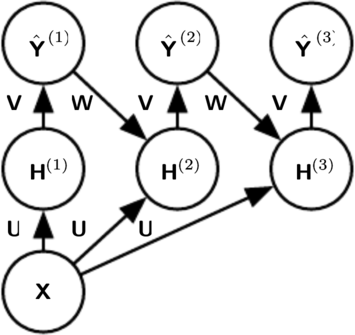
\includegraphics[scale=0.5]{images/86.png}}
\else
\centerline{\includegraphics{Chapter9/figures/iterative}}
\fi
\captionsetup{singlelinecheck=off}
\caption[.]{用于像素标记的\gls{recurrent_convolutional_network}的示例。
输入是图像张量$\TSX$,它的轴对应图像的行、列和通道(红,绿,蓝)。
目标是输出标签张量$\hat{Y}$,它遵循每个像素的标签的概率分布。
该张量的轴对应图像的行、列和不同类别。
\gls{recurrent_network}通过使用$\hat{Y}$的先前估计作为创建新估计的输入,来迭代地改善其估计,而不是单次输出$\hat{Y}$,。
每个更新的估计使用相同的参数,并且估计可以如我们所愿地被改善任意多次。
每一步使用的卷积核张量$\TSU$,是用来计算给定输入图像的隐藏表示的。
核张量$\TSV$用于产生给定隐藏值时标签的估计。
除了第一步之外,核$\TSW$都对$\hat{Y}$进行卷积来提供隐藏层的输入。
在第一步中,此项由零代替。
因为每一步使用相同的参数,所以这是一个\gls{recurrent_network}的例子,如\chapref{chap:sequence_modeling_recurrent_and_recursive_nets}所述。}
\label{fig:chap9_iterative}
\end{figure}

% -- 347 --
 
一旦对每个像素都进行了预测,我们就可以使用各种方法来进一步处理这些预测,以便获得图像在区域上的分割\citep{Briggman-et-al-NIPS2009,Turaga2010,Farabet-et-al-2013}。
一般的想法是假设大片相连的像素倾向于对应着相同的标签。
图模型可以描述相邻像素间的概率关系。
或者,\gls{convolutional_network}可以被训练来最大化地近似图模型的训练目标\citep{Ning-et-al-2005,Thompson-et-al-NIPS2014}。

\section{数据类型}
\label{sec:data_types}

\gls{convolutional_network}使用的数据通常包含多个通道,每个通道是时间上或空间中某一点的不同观测量。
参考表\,\ref{table:data_types}\,来了解具有不同维数和通道数的数据类型的例子。
 
% -- 348 --
\begin{table}[htbp!]
\centering
 \begin{tabular}[t]{l|p{0.4\textwidth}|p{0.4\textwidth}}
& 单通道 & 多通道\\ \hline
1维 & 
音频波形:卷积的轴对应于时间。我们将时间离散化并且在每个时间点测量一次波形的振幅。 &  
骨架动画(skeleton animation)数据:计算机渲染的3D角色动画是通过随时间调整``骨架''的姿势而生成的。 在每个时间点,角色的姿势通过骨架中的每个关节的角度来描述。我们输入到卷积模型的数据的每个通道,表示一个关节关于一个轴的角度。\\ \hline
2维 & 
已经使用\gls{Fourier_transform}预处理过的音频数据:我们可以将音频波形变换成2维张量,不同的行对应不同的频率,不同的列对应不同的时间点。在时间轴上使用卷积使模型等效于在时间上移动。在频率轴上使用卷积使得模型等效于在频率上移动,这使得在不同八度音阶中播放的相同旋律产生相同的表示,但处于网络输出中的不同高度。 & %Fourier transform这里不是很清楚,在频率上使用卷积是做什么的?
彩色图像数据:其中一个通道包含红色像素,另一个包含绿色像素,最后一个包含蓝色像素。在图像的水平轴和竖直轴上移动卷积核,赋予了两个方向上平移等变性。\\ \hline
3维 &
体积数据:这种数据一般来源于医学成像技术,例如CT扫描等。 & 
彩色视频数据:其中一个轴对应着时间,另一个轴对应着视频帧的高度,最后一个对应着视频帧的宽度。\\
\end{tabular}
\caption{用于\gls{convolutional_network}的不同数据格式的示例。}
\label{table:data_types}
\end{table}
% -- 349 --
 
\gls{convolutional_network}用于视频的例子,可以参考~\cite{Chen-Ting-2010}。

到目前为止,我们仅讨论了训练和测试数据中的每个样例都有相同的空间维度的情况。
\gls{convolutional_network}的一个优点是它们还可以处理具有可变的空间尺度的输入。
这些类型的输入不能用传统的基于矩阵乘法的神经网络来表示。
这为\gls{convolutional_network}的使用提供了令人信服的理由,即使当计算开销和过拟合都不是主要问题时。
%\footnote{译者注:传统的基于矩阵乘法的神经网络会面对计算开销和过拟合的问题,即使当计算开销和过拟合都不是主要问题时,我们也有充分的理由来使用卷积网络而不是传统的神经网络,因为卷积网络可以处理可变大小的输入。}

例如,考虑一组图像的集合,其中每个图像具有不同的高度和宽度。
目前还不清楚如何用固定大小的权重矩阵对这样的输入进行建模。
卷积就可以很直接地应用;核依据输入的大小简单地被使用不同次,并且卷积运算的输出也相应地放缩。
卷积可以被视为矩阵乘法;相同的卷积核为每种大小的输入引入了一个不同大小的\gls{doubly_block_circulant_matrix}。
有时,网络的输出允许和输入一样具有可变的大小,例如如果我们想要为输入的每个像素分配一个类标签。
在这种情况下,不需要进一步的设计工作。
在其他情况下,网络必须产生一些固定大小的输出,例如,如果我们想要为整个图像指定单个类标签。
在这种情况下,我们必须进行一些额外的设计步骤,例如插入一个\gls{pooling}层,\gls{pooling}区域的大小要与输入的大小成比例,以便保持固定数量的\gls{pooling}输出。
这种策略的一些例子可以参考\figref{fig:chap9_cnn_classifier}。

注意,使用卷积处理可变尺寸的输入,仅对输入是因为包含对同种事物的不同量的观察(时间上不同长度的记录,空间上不同宽度的观察等)而导致的尺寸变化这种情况才有意义。
如果输入是因为它可以选择性地包括不同种类的观察而具有可变尺寸,使用卷积是不合理的。
例如,如果我们正在处理大学申请,并且我们的特征包括成绩等级和标准化测试分数,但不是每个申请人都进行了标准化测试,则使用相同的权重来对成绩特征和测试分数特征进行卷积是没有意义的。

\section{高效的卷积算法}
\label{sec:efficient_convolution_algorithms}

现代\gls{convolutional_network}的应用通常需要包含超过百万个单元的网络。
利用并行计算资源的强大实现是很关键的,如\secref{sec:large_scale_deep_learning}中所描述的。
然而,在很多情况下,也可以通过选择适当的卷积算法来加速卷积。
 
% -- 350 --
 
卷积等效于使用\gls{Fourier_transform}将输入与核都转换到频域、执行两个信号的逐点相乘,再使用傅立叶逆变换转换回时域。
对于某些问题的规模,这种算法可能比离散卷积的朴素实现更快。

当一个$d$维的核可以表示成$d$个向量(每一维一个向量)的外积时,该核被称为\firstgls{separable}。
当核可分离时,朴素的卷积是低效的。
它等价于组合$d$个一维卷积,每个卷积使用这些向量中的一个。
组合方法显著快于使用它们的外积来执行一个$d$维的卷积。
并且核也只要更少的参数来表示成向量。
如果核在每一维都是$w$个元素宽,那么朴素的多维卷积需要$O(w^d)$的运行时间和参数存储空间,而可分离卷积只需要$O(w\times d)$的运行时间和参数存储空间。
当然,并不是每个卷积都可以表示成这种形式。

设计更快的执行卷积或近似卷积,而不损害模型准确性的方法,是一个活跃的研究领域。 
甚至仅提高\gls{forward_propagation}效率的技术也是有用的,因为在商业环境中,通常部署网络比训练网络还要耗资源。

\section{随机或无监督的特征}
\label{sec:random_or_unsupervised_features}

通常,\gls{convolutional_network}训练中最昂贵的部分是学习特征。 
输出层的计算代价通常相对不高,因为在通过若干层\gls{pooling}之后作为该层输入的特征的数量较少。
当使用梯度下降执行\gls{supervised}训练时,每步梯度计算需要完整地运行整个网络的前向传播和反向传播。
减少\gls{convolutional_network}训练成本的一种方式是使用那些不是由\gls{supervised}方式训练得到的特征。

有三种基本策略可以不通过\gls{supervised}训练而得到卷积核。
其中一种是简单地随机初始化它们。
另一种是手动设计它们,例如设置每个核在一个特定的方向或尺度来检测边缘。
最后,可以使用无监督的标准来学习核。
例如,\cite{Coates2011}将$k$均值聚类算法应用于小图像块,然后使用每个学得的中心作为卷积核。
第\ref{part:deep_learning_research}部分描述了更多的无监督学习方法。
使用无监督的标准来学习特征,允许这些特征的确定与位于网络结构顶层的分类层相分离。
然后只需提取一次全部训练集的特征,构造用于最后一层的新训练集。
假设最后一层类似\gls{logistic_regression}或者\,\glssymbol{SVM},那么学习最后一层通常是凸优化问题。

 
% -- 351 --
 
随机过滤器经常在\gls{convolutional_network}中表现得出乎意料得好~\cite{Jarrett-ICCV2009,Saxe-ICML2011,pinto2011scaling,cox2011beyond}。
\cite{Saxe-ICML2011}~说明,由卷积和随后的\gls{pooling}组成的层,当赋予随机权重时,自然地变得具有频率选择性和平移不变性。
他们认为这提供了一种廉价的方法来选择\gls{convolutional_network}的结构:首先通过仅训练最后一层来评估几个\gls{convolutional_network}结构的性能,然后选择最好的结构并使用更昂贵的方法来训练整个网络。

一个中间方法是学习特征,但是使用那种不需要在每个梯度计算步骤中都进行完整的前向和反向传播的方法。
与多层感知机一样,我们使用\gls{greedy_layer_wise_pretraining},单独训练第一层,然后一次性地从第一层提取所有特征,之后用那些特征单独训练第二层,以此类推。
\chapref{chap:optimization_for_training_deep_models}描述了如何实现\gls{supervised}的\gls{greedy_layer_wise_pretraining},第\ref{part:deep_learning_research}部分将此扩展到了无监督的范畴。
卷积模型的\gls{greedy_layer_wise_pretraining}的经典模型是卷积\gls{DBN}\citep{HonglakL2009}。
\gls{convolutional_network}为我们提供了相对于多层感知机更进一步采用预训练策略的机会。
并非一次训练整个卷积层,我们可以训练一小块模型,就像~\cite{Coates2011}使用$k$均值做的那样。
然后,我们可以用来自这个小块模型的参数来定义卷积层的核。
这意味着使用无监督学习来训练\gls{convolutional_network}\emph{并且在训练的过程中完全不使用卷积}是可能的。
使用这种方法,我们可以训练非常大的模型,并且只在推断期间产生高计算成本\citep{ranzato-cvpr-07-small,Jarrett-ICCV2009,koray-nips-10-small,icml2013_coates13}。
这种方法大约在2007到2013年间流行,当时标记的数据集很小,并且计算能力有限。
如今,大多数\gls{convolutional_network}以纯粹\gls{supervised}的方式训练,在每次训练迭代中使用通过整个网络的完整的前向和反向传播。
 
% -- 352 --
 
与其他无监督预训练的方法一样,使用这种方法的一些好处仍然难以说清。
无监督预训练可以提供一些相对于\gls{supervised}训练的正则化,或者它可以简单地允许我们训练更大的结构,因为它的学习规则降低了计算成本。

\section{\glsentrytext{convolutional_network}的神经科学基础}
\label{sec:the_neuroscientific_basis_for_convolutional_networks}

\gls{convolutional_network}也许是生物学启发人工智能的最为成功的案例。
虽然\gls{convolutional_network}也经过许多其他领域的指导,但是神经网络的一些关键设计原则来自于神经科学。

\gls{convolutional_network}的历史始于神经科学实验,远早于相关计算模型的发展。
为了确定关于哺乳动物视觉系统如何工作的许多最基本的事实,神经生理学家David Hubel和Torsten Wiesel合作多年\citep{Hubel+Wiesel-1959,Hubel62,Hubel+Wiesel-1968}。
他们的成就最终获得了诺贝尔奖。
他们的发现对当代深度学习模型有最大影响的是基于记录猫的单个神经元的活动。
他们观察了猫的脑内神经元如何响应投影在猫前面屏幕上精确位置的图像。
他们的伟大发现是,处于视觉系统较为前面的神经元对非常特定的光模式(例如精确定向的条纹)反应最强烈,但对其他模式几乎完全没有反应。

他们的工作有助于表征大脑功能的许多方面,这些方面超出了本书的范围。
从深度学习的角度来看,我们可以专注于简化的、草图形式的大脑功能视图。

在这个简化的视图中,我们关注被称为V1的大脑的一部分,也称为\firstgls{primary_visual_cortex}。
V1是大脑对视觉输入开始执行显著高级处理的第一个区域。
在该草图视图中,图像是由光到达眼睛并刺激视网膜(眼睛后部的光敏组织)形成的。
视网膜中的神经元对图像执行一些简单的预处理,但是基本不改变它被表示的方式。
然后图像通过视神经和称为\emph{外侧膝状核}的脑部区域。 
这些解剖区域的主要作用是仅仅将信号从眼睛传递到位于头后部的V1。
 
% -- 353 --
 
\gls{convolutional_network}层被设计为描述V1的三个性质:
\begin{enumerate}
  \item V1可以进行空间映射。
  %这里翻译不好
  它实际上具有二维结构来反映视网膜中的图像结构。
  例如,到达视网膜下半部的光仅影响V1相应的一半。 
  \gls{convolutional_network}通过用二维映射定义特征的方式来描述该特性。

  \item V1包含许多\firstgls{simple_cells}。
  简单细胞的活动在某种程度上可以概括为在一个小的空间位置感受野内的图像的线性函数。
  \gls{convolutional_network}的检测器单元被设计为模拟简单细胞的这些性质。

  \item V1还包括许多\firstgls{complex_cells}。
  这些细胞响应类似于由简单细胞检测的那些特征,但是复杂细胞对于特征的位置微小偏移具有不变性。 
  这启发了\gls{convolutional_network}的\gls{pooling}单元。
  复杂细胞对于照明中的一些变化也是不变的,不能简单地通过在空间位置上\gls{pooling}来刻画。 
  这些不变性激发了\gls{convolutional_network}中的一些跨通道\gls{pooling}策略,例如maxout单元\citep{Goodfellow-et-al-ICML2013}。
\end{enumerate}

虽然我们最了解V1,但是一般认为相同的基本原理也适用于视觉系统的其他区域。
在我们视觉系统的草图视图中,当我们逐渐深入大脑时,遵循\gls{pooling}的基本探测策略被反复执行。
当我们穿过大脑的多个解剖层时,我们最终找到了响应一些特定概念的细胞,并且这些细胞对输入的很多种变换都具有不变性。
这些细胞被昵称为``祖母细胞''——这个想法是一个人可能有一个神经元,当看到他祖母的照片时该神经元被激活,无论祖母是出现在照片的左边或右边,无论照片是她的脸部的特写镜头还是她的全身照,也无论她处在光亮还是黑暗中,等等。

这些祖母细胞已经被证明确实存在于人脑中,在一个被称为\emph{内侧颞叶}的区域\citep{quiroga2005invariant}。
研究人员测试了单个神经元是否会响应名人的照片。
他们发现了后来被称为``Halle Berry神经元''的神经元:由Halle Berry的概念激活的单个神经元。
当一个人看到Halle Berry的照片,Halle Berry的图画,甚至包含单词``Halle Berry''的文本时,这个神经元会触发。
当然,这与Halle Berry本人无关;其他神经元会对Bill Clinton,Jennifer Aniston等的出现做出响应。
 
% -- 354 --
 
这些内侧颞叶神经元比现代\gls{convolutional_network}更通用一些,这些网络在读取名称时不会自动联想到识别人或对象。
与\gls{convolutional_network}的最后一层在特征上最接近的类比是称为\emph{颞下皮质}(IT)的脑区。
当查看一个对象时,信息从视网膜经LGN流到V1,然后到V2,V4,之后是IT。
这发生在瞥见对象的前100ms内。
如果允许一个人继续观察对象更多的时间,那么信息将开始回流,因为大脑使用自上而下的反馈来更新较低级脑区中的激活。
然而,如果我们打断人的注视,并且只观察前100ms内的大多数前向激活导致的放电率,那么IT被证明与\gls{convolutional_network}非常相似。
\gls{convolutional_network}可以预测IT放电率,并且在执行对象识别任务时与人类(时间有限的情况)非常类似\citep{dicarlo-tutorial-2013}。

话虽如此,\gls{convolutional_network}和哺乳动物的视觉系统之间还是有许多区别。
这些区别有一些是计算神经科学家所熟知的,但超出了本书的范围。
还有一些区别尚未知晓,因为关于哺乳动物视觉系统如何工作的许多基本问题仍未得到回答。
简要列表如下:
\begin{itemize}
  \item 人眼大部分是非常低的分辨率,除了一个被称为\firstgls{fovea}的小块。
  中央凹仅观察在手臂长度距离内一块拇指大小的区域。
  虽然我们觉得我们可以看到高分辨率的整个场景,但这是由我们的大脑的潜意识部分创建的错觉,因为它缝合了我们瞥见的若干个小区域。
  大多数\gls{convolutional_network}实际上接收大的全分辨率的照片作为输入。
  人类大脑控制几次眼动,称为\firstgls{saccade},以瞥见场景中最显眼的或任务相关的部分。
  将类似的\gls{attention_mechanism}融入深度学习模型是一个活跃的研究方向。
  在深度学习的背景下,\gls{attention_mechanism}对于自然语言处理是最成功的,参考\secref{sec:using_an_attention_mechanism_and_aligning_pieces_of_data}。
  研究者已经研发了几种具有视觉机制的视觉模型,但到目前为止还没有成为主导方法\citep{Larochelle2010,Denil2012}。
  
  \item 人类视觉系统集成了许多其他感觉,例如听觉,以及像我们的心情和想法一样的因素。
  \gls{convolutional_network}迄今为止纯粹是视觉的。
  
  \item 人类视觉系统不仅仅用于识别对象。
  它能够理解整个场景,包括许多对象和对象之间的关系,以及处理我们的身体与世界交互所需的丰富的三维几何信息。
  \gls{convolutional_network}已经应用于这些问题中的一些,但是这些应用还处于起步阶段。
  
  \item 即使像V1这样简单的大脑区域也受到来自较高级别的反馈的严重影响。
  反馈已经在神经网络模型中被广泛地探索,但还没有被证明提供了引人注目的改进。
  
  \item 虽然前馈IT放电频率刻画了与\gls{convolutional_network}特征很多相同的信息,但是仍不清楚中间计算的相似程度。
  大脑可能使用非常不同的激活和\gls{pooling}函数。
  单个神经元的激活可能不能用单个线性过滤器的响应来很好地表征。
  最近的V1模型涉及对每个神经元的多个二次过滤器\citep{rust:2005}。
  事实上,我们的``简单细胞''和``复杂细胞''的草图图片可能并没有区别;简单细胞和复杂细胞可能是相同种类的细胞,但是它们的``参数''使得它们能够实现从我们所说的``简单''到``复杂''的连续的行为。
\end{itemize}
 
% -- 355 --
 
还值得一提的是,神经科学很少告诉我们该如何\emph{训练}\gls{convolutional_network}。
具有跨多个空间位置的\gls{parameter_sharing}的模型结构,可以追溯到早期关于视觉的联结主义模型\citep{Marr76},但是这些模型没有使用现代的反向传播算法和梯度下降。
例如,\citep{Fukushima80}结合了现代\gls{convolutional_network}的大多数模型结构设计元素,但依赖于层次化的无监督聚类算法。

\cite{Lang+Hinton88}引入反向传播来训练\firstall{TDNNs}。
使用当代术语来说,TDNN是用于时间序列的一维\gls{convolutional_network}。
用于这些模型的反向传播不受任何神经科学观察的启发,并且被一些人认为是生物不可信的。
在基于使用反向传播训练的TDNN成功之后,\cite{LeCun89d}通过将相同的训练算法应用于图像的2维卷积来发展现代\gls{convolutional_network}。

到目前为止,我们已经描述了简单细胞对于某些特征是如何呈现粗略的线性和选择性,复杂细胞是如何更加的非线性,并且对于这些简单细胞特征的某些变换具有不变性,以及在选择性和不变性之间交替放置的层可以产生对非常特定现象的祖母细胞。
我们还没有精确描述这些单个细胞检测到了什么。
在深度非线性网络中,可能难以理解单个细胞的功能。
第一层中的简单细胞相对更容易分析,因为它们的响应由线性函数驱动。
在人工神经网络中,我们可以直接显示卷积核的图像,来查看卷积层的相应通道是如何响应的。
在生物神经网络中,我们不能访问权重本身。
相反,我们在神经元自身中放置一个电极,在动物视网膜前显示几个白噪声图像样本,并记录这些样本中的每一个是如何导致神经元激活的。
然后,我们可以对这些响应拟合线性模型,以获得近似的神经元权重。
这种方法被称为\firstgls{reverse_correlation}\citep{ringach2004reverse}。
 
% -- 356 --
 
\gls{reverse_correlation}向我们表明,大多数的V1细胞具有由\firstgls{Gabor_function}所描述的权重。
\gls{Gabor_function}描述在图像中的2维点处的权重。我们可以认为图像是2维坐标$I(x,y)$的函数。
类似地,我们可以认为简单细胞是在图像中的一组位置采样,这组位置由一组$x$坐标$\SetX$和一组$y$坐标$\SetY$来定义,并且使用的权重$w(x,y)$也是位置的函数。
从这个观点来看,简单细胞对于图像的响应由下式给出
\begin{equation}
  s(I)=\sum_{x\in \SetX} \sum_{y\in \SetY} w(x, y)I(x,y).
\end{equation}
特别地,$w(x,y)$采用\gls{Gabor_function}的形式:
\begin{equation}
  w(x, y; \alpha, \beta_x, \beta_y, f, \phi, x_0, y_0, \tau) = \alpha \exp(-\beta_x x'^2 - \beta_y y'^2) \cos (fx' + \phi),
\end{equation}
其中
\begin{equation}
  x' = (x-x_0)\cos(\tau) + (y-y_0)\sin(\tau)
\end{equation}
以及
\begin{equation}
  y' = -(x-x_0) \sin(\tau) + (y-y_0)\cos(\tau).
\end{equation}

这里$\alpha, \beta_x, \beta_y, f, \phi, x_0, y_0, \tau$都是控制~\gls{Gabor_function}性质的参数。
\figref{fig:chap9_Gabor_functions}给出了\gls{Gabor_function}在不同参数集上的一些例子。
% fig 9.18
\begin{figure}
\ifOpenSource
\centerline{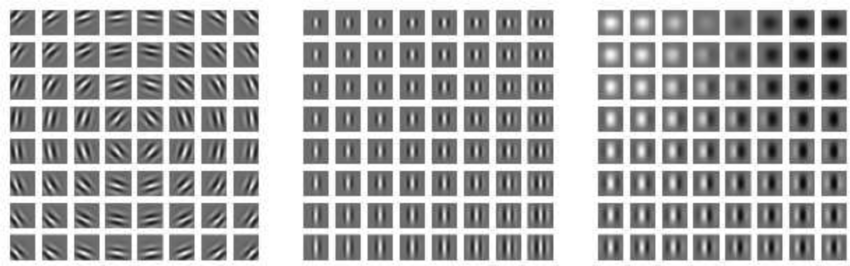
\includegraphics[scale=0.5]{images/87.png}}
\else
\centering    
\subfigure{ \label{fig:chap9_Gabor_functions_a}     
\includegraphics[width=0.3\textwidth]{Chapter9/figures/gabor_sinusoid.png}}     
\subfigure{ \label{fig:chap9_Gabor_functions_b}     
\includegraphics[width=0.3\textwidth]{Chapter9/figures/gabor_coordinate_system.png}}
\subfigure{ \label{fig:chap9_Gabor_functions_c}     
\includegraphics[width=0.3\textwidth]{Chapter9/figures/gabor_scale.png}}     
\fi
\captionsetup{singlelinecheck=off}
\caption{具有各种参数设置的\gls{Gabor_function}。
白色表示大的正权重,黑色表示大的负权重,背景灰色对应于零权重。
\emph{(左)}控制坐标系的参数具有不同值的\gls{Gabor_function},这些参数包括:$x_0$、$y_0$和$\gamma$。
在该网格中的每个\gls{Gabor_function}被赋予和它在网格中的位置成比例的$x_0$和$y_0$的值,并且$\tau$被选择为使得每个Gabor过滤器对从网格中心辐射出的方向非常敏感。
对于其他两幅图,$x_0$、$y_0$和$\gamma$固定为零。
\emph{(中)}具有不同高斯比例参数$\beta_x$和$\beta_y$的\gls{Gabor_function}。
当我们从左到右通过网格时,\gls{Gabor_function}被设置为增加宽度(减少$\beta_x$);当我们从上到下通过网格时,\gls{Gabor_function}被设置为为增加高度(减少$\beta_y$)。
对于其他两幅图,$\beta$值固定为图像宽度的1.5倍。
\emph{(右)}具有不同的正弦参数$f$和$\phi$的\gls{Gabor_function}。
当我们从上到下移动时,$f$增加;当我们从左到右移动时,$\phi$增加。对于其他两幅图,$\phi$固定为0,$f$固定为图像宽度的5倍。}     
\label{fig:chap9_Gabor_functions}     
\end{figure}

参数$x_0,y_0$和$\tau$定义坐标系。
我们平移和旋转$x$和$y$来得到$x'$和$y'$。
具体地,简单细胞会响应以点$(x_0, y_0)$为中心的图像特征,并且当我们沿着从水平方向旋转$\tau$弧度的线移动时,简单细胞将响应亮度的变化。
 
% -- 357 --
 
作为$x'$和$y'$的函数,函数$w$会响应当我们沿着$x'$移动时的亮度变化。
它有两个重要的因子:一个是高斯函数,另一个是余弦函数。

高斯因子$ \alpha \exp(-\beta_x x'^2 - \beta_y y'^2)$可以被视为阈值项,用于保证简单细胞仅对接近$x'$和$y'$都为零点处的值响应,换句话说,接近细胞接受域的中心。
尺度因子$\alpha$调整简单细胞响应的总的量级,而$\beta_x$和$\beta_y$控制接受域消退的速度。

余弦因子$ \cos (fx' + \phi)$控制简单细胞如何响应延$x‘$轴的亮度改变。
参数$f$控制余弦的频率,$\phi$控制它的相位偏移。

合在一起,简单细胞的这个草图视图意味着,简单细胞对在特定位置处、特定方向上、特定空间频率的亮度进行响应。
当图像中的光波与细胞的权重具有相同的相位时,简单细胞是最兴奋的。
这种情况发生在当图像亮时,它的权重为正,而图像暗时,它的权重为负。
当光波与权重完全异相时,简单细胞被抑制——当图像较暗时,它的权重为正;较亮时,它的权重为负。
 
% -- 358 --
 
复杂细胞的草图视图是它计算包含两个简单细胞响应的2维向量的$L^2$范数:$c(I)=\sqrt{s_0(I)^2 + s_1(I)^2}$。
一个重要的特殊情况是当$s_1$和$s_0$具有除$\phi$ 以外都相同的参数,并且$\phi$被设置为使得$s_1$与$s_0$相位相差四分之一周期时。
在这种情况下,$s_0$和$s_1$形成\firstgls{quadrature_pair}。
当高斯重新加权的图像$I(x,y)\exp(-\beta_x x'^2 -\beta_y y^2)$包含具有频率$f$、在方向$\tau$上、接近$(x_0, y_0)$的高振幅正弦波时,用先前方法定义的复杂细胞会响应,并且\emph{不管该波的相位偏移}。
换句话说,复杂细胞对于图像在方向$\tau$上的微小变换或者翻转图像(用白色代替黑色,反之亦然)具有不变性。

神经科学和机器学习之间最显著的对应关系,是从视觉上比较机器学习模型学得的特征与使用V1得到的特征。
\cite{Olshausen+Field-1996}说明,一个简单的无监督学习算法,稀疏编码,学习的特征具有与简单细胞类似的感受野。
从那时起,我们发现,当应用于自然图像时,极其多样的统计学习算法学习类\gls{Gabor_function}的特征。这包括大多数深度学习算法,它们在其第一层中学习这些特征。
\figref{fig:chap9_feature_detectors}给出了一些例子。
因为如此众多不同的学习算法学习边缘检测器,所以很难仅基于学习算法学得的特征,来断定哪一个特定的学习算法是``正确''的大脑模型(虽然,当应用于自然图像时,如果一个算法\emph{不能}学得某种检测器时,它能够作为一种否定标志)。
这些特征是自然图像的统计结构的重要部分,并且可以通过许多不同的统计建模方法来重新获得。
读者可以参考\citep{hyvarinen-book2009}来获得自然图像统计领域的综述。
% fig 9.19
\begin{figure}
\ifOpenSource
\centerline{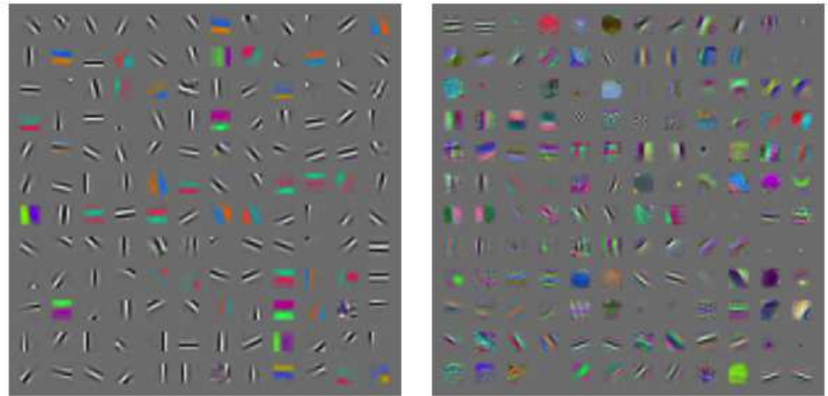
\includegraphics[scale=0.5]{images/88.png}}
\else
\centering    
\subfigure{ \label{fig:chap9_feature_detectors_a}     
\includegraphics[width=0.4\textwidth]{Chapter9/figures/maxout_kernels.png}}     
\subfigure{ \label{fig:chap9_feature_detectors_b}     
\includegraphics[width=0.4\textwidth]{Chapter9/figures/s3c_filters.png}}    
\fi
\caption{许多机器学习算法在应用于自然图像时,会学习那些用来检测边缘或边缘的特定颜色的特征。 
这些特征检测器使人联想到已知存在于初级视觉皮层中的~\gls{Gabor_function}。   
\emph{(左)}通过应用于小图像块的无监督学习算法(\gls{ss}稀疏编码)学得的权重。%这里不是很懂
\emph{(右)}由完全\gls{supervised}的卷积~\gls{maxout}~网络的第一层学得的卷积核。 相邻的一对过滤器驱动相同的~\gls{maxout_unit}。}     
\label{fig:chap9_feature_detectors}     
\end{figure}

\section{卷积网络与深度学习的历史}
\label{sec:convolutional_networks_and_the_history_of_deep_learning}
 
% -- 359 --
 
\gls{convolutional_network}在深度学习的历史中发挥了重要作用。
它们是将研究大脑获得的深刻理解成功用于机器学习应用的关键例子。
它们也是第一个表现良好的深度模型之一,远远早于任意深度模型被认为是可行的。
\gls{convolutional_network}也是第一个解决重要商业应用的神经网络,并且仍然是当今深度学习商业应用的前沿。
例如,在20世纪90年代,AT\&T的神经网络研究小组开发了一个用于读取支票的\gls{convolutional_network}\citep{chapter-gradient-document-2001}。
到90年代末,NEC部署的这个系统已经被用于读取美国10%以上的支票。
后来,微软部署了若干个基于\gls{convolutional_network}的OCR和手写识别系统\citep{simard-03-small}。 
关于\gls{convolutional_network}的这种应用和更现代应用的更多细节,参考\chapref{chap:applications}。
读者可以参考\citep{lecun_convolutional_2010}了解2010年之前的更为深入的\gls{convolutional_network}历史。

\gls{convolutional_network}也被用作在许多比赛中的取胜手段。
当前对深度学习的商业兴趣的热度始于\cite{Krizhevsky-2012}赢得了ImageNet对象识别挑战,但是在那之前,\gls{convolutional_network}也已经被用于赢得前些年影响较小的其他机器学习和计算机视觉竞赛了。
 
% -- 360 --
 
\gls{convolutional_network}是第一批能使用反向传播有效训练的的深度网络之一。
现在仍不完全清楚为什么\gls{convolutional_network}在一般的反向传播网络被认为已经失败时反而成功了。
这可能可以简单地归结为\gls{convolutional_network}比全连接网络计算效率更高,因此使用它们运行多个实验并调整它们的实现和超参数更容易。
更大的网络也似乎更容易训练。
利用现代硬件,大型全连接的网络在许多任务上也表现得很合理,即使使用过去那些全连接网络被认为不能工作得很好的数据集和当时流行的激活函数时,现在也能执行得很好。
心理可能神经网络成功的主要阻碍(实践者没有期望神经网络有效,所以他们没有认真努力地使用神经网络)。
无论如何,幸运的是\gls{convolutional_network}在几十年前就表现良好。
在许多方面,它们为余下的深度学习传递火炬,并为一般的神经网络被接受铺平了道路。

\gls{convolutional_network}提供了一种方法来特化神经网络,使其能够处理具有清楚的网格结构拓扑的数据,以及将这样的模型扩展到非常大的规模。 
这种方法在二维图像拓扑上是最成功的。
为了处理一维序列数据,我们接下来转向神经网络框架的另一种强大的特化:\gls{RNN}。

 
% -- 361 --
 










